% =====================================================================
% Chapter I.3: Observables II: defects and extended operators
% =====================================================================
\section{Observables II: defects and extended operators}
\label{ch:extended-operators}

Chapter I.2 closed with a warning attached to its own title: the local data,
complete as it is on its own terms, does not exhaust the observables of a
quantum field theory. This chapter is about the observables it misses ---
operators supported not at points but on lines, surfaces, and
higher-dimensional submanifolds of spacetime, together with the boundaries
and interfaces that are their codimension-one extreme --- and its thesis is
the lesson the subject absorbed between roughly 2014 and 2026: \emph{the
extended operators are part of the definition of the theory}. They are not
composites of local operators, not bookkeeping for sources, and not
optional decorations; they are an independent column of chapter I.1's
inventory (item 4 of Definition~\ref{def:inventory}), and two theories can
agree on every correlator of every local operator on $\reals^d$ and still
differ --- in their physics, not merely in their presentation --- because
they differ in their extended operators. Chapter I.1's
Exercise~\ref{exr:two-theories-same-correlators} asked the reader to hold
exactly this possibility in mind; this chapter makes good on it, with
four-dimensional gauge theories supplying the canonical
example.\footnote{Aharony--Seiberg--Tachikawa \arxiv{1305.0318}, whose title
--- \emph{Reading between the lines of four-dimensional gauge theories} ---
states the conclusion exactly: the missing data lives in the lines.}

\begin{qquestion}
What observables live on submanifolds of spacetime? How are they defined
when no Lagrangian is given --- and when one is? Is the extended-operator
content determined by the local data, and if not, what physics does it
carry that local correlators cannot: which symmetries act on it, which
phases does it diagnose, which Hilbert spaces does it create?
\end{qquestion}

\noin The reader has met extended operators before, although the textbook
treatment makes them easy to mistake for technical devices. The Wilson loop
appears in a gauge-theory course as a gauge-invariant functional useful for
discussing confinement; boundary conditions appear as something one imposes
to make a problem well-posed; the disorder operator of the Ising model, if
it appears at all, appears as a trick of the duality literature. The modern
view assembles these scattered objects into a single structural statement.
A quantum field theory assigns data not only to points of spacetime but to
embedded submanifolds of every dimension, and this assignment is constrained,
organized, and physical: constrained by mutual locality (two extended
operators must be insertable in the same correlator unambiguously),
organized by codimension and by the symmetries that act, and physical in
that the long-distance behavior of extended operators distinguishes phases
that no local order parameter can tell apart. The last point is the oldest:
it is Wilson's 1974 criterion for confinement,\footnote{K.~G.~Wilson,
\emph{Confinement of quarks}, Phys.\ Rev.\ D \textbf{10} (1974) 2445 ---
the paper that introduced both lattice gauge theory and the loop
observable now bearing his name, for exactly this diagnostic purpose.} and
the newest developments of Part II --- where symmetries themselves become
topological extended operators, and the objects they act on are lines and
surfaces --- stand directly on it.

The chapter runs as follows. We first say what an extended operator
\emph{is}, which requires confronting the same question chapter I.2
confronted for local operators: the naive constructions (integrate a local
density along a curve; impose a constraint) are presentations, and the
object itself must be characterized by its correlators. Doing this
carefully produces a division of all extended operators into two
construction types --- \vocab{order}-type, built from the fields of a
presentation, and \vocab{disorder}-type, defined by prescribing a
singularity --- and a sharper division, independent of any presentation,
into \vocab{genuine} operators and operators attached to something of one
dimension higher. The chapter's centerpiece then builds the oldest
disorder operator in physics, the Kramers--Wannier disorder line of the
two-dimensional Ising model, entirely on the lattice, where every claim is
a finite computation: the line will be constructed, proved topological,
dualized, and used to diagnose both phases of the model --- and at the
critical point it will manufacture a fermion out of bosonic spins. With
this concrete case in hand we turn to gauge theories, where the same
order/disorder pair becomes the Wilson/'t~Hooft pair, and where the
celebrated result of Aharony--Seiberg--Tachikawa shows that choosing the
mutually local set of lines is part of choosing the theory. Two further
sections develop what defects do once they exist: as \emph{probes}, they
acquire conformal data of their own (one-point functions, defect-localized
operators, the displacement operator) --- the kinematics of defect CFT,
with boundaries as the richest case; as \emph{sources of states}, they
define new Hilbert spaces --- the defect (twisted) Hilbert spaces whose
necessity chapter I.2's closing already hinted at, and which chapter I.4's
cutting-and-gluing formalism will absorb as just more geometry.

Throughout, ``defect'' and ``extended operator'' are synonyms, used
interchangeably as the literature does;\footnote{There is a habit, harmless
once stated, of saying \emph{operator} when the object sits at fixed time
and acts on a Hilbert space, and \emph{defect} when it extends in the time
direction and modifies the Hilbert space. In Euclidean signature the two
configurations are rotations of one another, and the distinction is one of
frame, not of substance; Section~\ref{sec:defect-hilbert} exploits the
rotation. The usage follows Gaiotto--Kapustin--Seiberg--Willett
\arxiv{1412.5148}, \S1.} the convention pays off in
Section~\ref{sec:defect-hilbert}, where rotating an extended operator from
``space'' into ``time'' is the chapter's final tool.

% =====================================================================
\subsection{What is an extended operator?}
\label{sec:what-is-defect}

Chapter I.2 opened by asking what a local operator is, and found that
the durable answer bypasses fields: a local operator is whatever has
well-defined correlation functions at a point, with the set of such objects
constructed by organizing coincident-point singularities or by
diagonalizing the renormalization group. The same discipline applies one
dimension up, and since the rest of the chapter rests on it, we state it
as a definition. Defining by correlators, rather than by any particular
construction, is what makes the notion presentation-independent --- the
same reason chapter I.2's Definition~\ref{def:local-operator} was phrased
as it was --- and it is what will allow the dualities met below to map
extended operators built in one presentation onto extended operators
built, by entirely different means, in another.

\begin{ddefinition}[Extended operator]
\label{def:extended-operator}
An \vocab{extended operator} (synonymously, a \vocab{defect}) supported
on a $p$-dimensional submanifold $\Sigma_p \subset M_d$ is an object
$V(\Sigma_p)$ with well-defined correlation functions
\begin{equation}
\left\langle V(\Sigma_p)\, \op_1(x_1) \cdots \op_n(x_n) \right\rangle
\label{eq:defect-correlator}
\end{equation}
jointly with the local operators and with other extended operators. The
\vocab{extended-operator content} of a theory is the list of all such
$V$, for each $p$, that the theory admits --- item 4 of chapter I.1's
inventory (Definition~\ref{def:inventory}), now with the same standing
as the local operator content.
\end{ddefinition}

\noin As with local operators, the useful question is how such objects
are \emph{constructed} in the presentations we own. There are two
constructions, and the difference between them organizes everything that
follows.

\subsubsection{Order-type: couple something to the submanifold}
\label{sec:order-type}

The first construction is transparent: build the extended operator out of
the fields of the presentation. The mildest version inserts the integral of
a local operator along $\Sigma_p$ into the path integral, exponentiated so
that the insertion resembles a source term in the action,
\begin{equation}
V_h(\Sigma_p) = \exp\left( h \int_{\Sigma_p} d^p\sigma\, \op(\sigma) \right),
\label{eq:order-defect}
\end{equation}
for some local operator $\op$ and coupling $h$. Physically this is an
\emph{impurity}: the theory in the bulk is undisturbed, but along
$\Sigma_p$ the action has been modified. A magnetic field applied along a
line in a magnet, a charged particle's worldline in an electromagnetic
field, a localized chemical potential --- all are insertions of the form
\eqref{eq:order-defect}. More elaborate versions place new degrees of
freedom on $\Sigma_p$ --- a quantum-mechanical spin sitting on a worldline
(the Kondo impurity), a full $p$-dimensional field theory living on the
defect and coupled to the bulk fields --- but the principle is the same:
everything is built from ingredients the presentation already supplies,
locally along the defect. Operators of this construction type are called
\vocab{order}-type defects. The name is retrospective, chosen for contrast
with what comes next, and the Wilson line of
Section~\ref{sec:gauge-lines} is its most consequential instance.

Even this mild construction produces objects that are not local operators
in disguise, and it is instructive to see how in the simplest possible
case.

\begin{eexample}[The simplest defect: a static impurity in a free field]
\label{ex:static-impurity}
Take the free massless scalar in $d = 4$ Euclidean dimensions,
normalized as in chapter I.2 with
$\langle\phi(x)\phi(0)\rangle = \frac{1}{4\pi^2 x^2}$, and insert the
line defect \eqref{eq:order-defect} along the straight line
$\Sigma_1 = \{(\tau, \mathbf{0})\}$ --- the Euclidean worldline of a
static pointlike impurity coupled linearly to $\phi$:
\begin{equation}
V_h = \exp\left( h \int_{-\infty}^{\infty} d\tau\, \phi(\tau, \mathbf{0})\right).
\end{equation}
The theory is Gaussian, so every correlator in the presence of $V_h$ can
be computed by completing the square: inserting $V_h$ shifts $\phi$ by
the classical field of the source. The simplest output is the one-point
function of $\phi$ itself, which without the defect would vanish.
At distance $r = |\mathbf{x}|$ from the line,
\begin{equation}
\left\langle \phi(x) \right\rangle_{V_h}
\equiv \frac{\left\langle \phi(x)\, V_h \right\rangle}{\left\langle V_h \right\rangle}
= h \int_{-\infty}^{\infty} d\tau\,
\frac{1}{4\pi^2\left[(x_0-\tau)^2 + r^2\right]}
= \frac{h}{4\pi r}:
\label{eq:impurity-onepoint}
\end{equation}
the Coulomb profile of a static charge, here derived as the response of
the vacuum to a line operator. The computation is two lines long, but
it carries structural lessons that generalize far beyond free fields.
First, a defect gives one-point functions to operators that had none:
the defect breaks the symmetries (here translations and rotations
transverse to the line) that forced $\langle\phi\rangle = 0$, and the
surviving symmetry --- translations along the line, rotations around it,
and, since $h\int\phi\, d\tau$ is dimensionless in $d=4$, dilatations
centered on the line --- fixes the answer to be a pure power of the
transverse distance, $\langle\op\rangle_V = a_{\op}/r^{\Delta}$. The
coefficient $a_\phi = h/4\pi$ is new data, not contained in the bulk
correlators; Section~\ref{sec:defect-cft} promotes such coefficients to
the front rank of observables. Second, the defect requires
renormalization of its own. The normalization $\langle V_h\rangle$
contains the integral $\frac{h^2}{2}\int d\tau\, d\tau'\,
\langle\phi(\tau)\phi(\tau')\rangle$, which diverges at $\tau \to \tau'$
--- a divergence proportional to the \emph{length} of the line, removed
by a counterterm $\delta m \int d\tau$ on the worldline, i.e.\ a
renormalization of the impurity's rest energy. Defect couplings run,
defect operators acquire anomalous dimensions, and there is a defect
renormalization group, with fixed points and all (it returns in
Section~\ref{sec:defect-cft} and, as a tool for solving impurity
problems, in Part III.5). Third, nothing about $V_h$ is a local operator
in disguise: no sum of local insertions reproduces an object whose
correlators decay as a power of the distance \emph{to a line}. The
defect is a new entry in the inventory, even in a free theory.
\end{eexample}

\begin{exercise}[easy]
\label{exr:impurity-general-d}
(The impurity in general dimension.) Repeat the computation
\eqref{eq:impurity-onepoint} for the free massless scalar in general $d$
(two-point function $\langle\phi(x)\phi(0)\rangle = \frac{c_d}{x^{d-2}}$
with $c_d = \frac{\Gamma(d/2-1)}{4\pi^{d/2}}$): show that
\begin{equation*}
\left\langle \phi(r) \right\rangle_{V_h} = h\, c_d\, b_d\, r^{3-d},
\qquad
b_d = \int_{-\infty}^\infty \frac{du}{(1+u^2)^{(d-2)/2}},
\end{equation*}
convergent for $d > 3$. The exponent $d - 3$ agrees with $\Delta_\phi =
\frac{d-2}{2}$ only at $d = 4$; explain the mismatch (the coupling $h$
is dimensionful away from $d = 4$ and supplies the missing power), and
conclude that the line defect \eqref{eq:order-defect} built from $\phi$
is scale-invariant exactly in $d = 4$, relevant (growing toward the
infrared) for $d < 4$, and irrelevant for $d > 4$ --- the defect
renormalization group in its simplest instance.
\hint{Power counting on the worldline: the integrated operator
$\int d\tau\, \op$ is a marginal defect coupling when $\Delta_\op = p
= 1$. The relevant case $d = 3$ is physical: a localized magnetic field
in the 3d Ising model, the ``pinning defect,'' flows to a nontrivial
defect fixed point analyzed in Cuomo--Komargodski--Mezei
\texttt{2112.10634}.}
\answ{$\langle\phi(r)\rangle_{V_h} = h c_d r^{3-d} b_d$ by the
substitution $\tau = r u$; for $d=4$, $c_4 = 1/4\pi^2$ and $b_4 = \pi$
reproduce \eqref{eq:impurity-onepoint}.}
\end{exercise}

\subsubsection{Disorder-type: prescribe a singularity}
\label{sec:disorder-type}

The second construction is the one with no analogue among naive
composites, and it is the reason extended operators cannot be derived from
the local data. Instead of \emph{adding} something along $\Sigma_p$, one
\emph{removes} $\Sigma_p$ from spacetime and instructs the path integral to
sum only over field configurations with a prescribed singularity --- a
prescribed winding, holonomy, or flux --- around the excised locus. No new
term is added to the action; the definition modifies the \emph{space of
configurations} rather than the weight. Operators of this construction
type are called \vocab{disorder}-type defects, or disorder operators.

The prototype predates gauge theory. In a theory with a compact scalar ---
a field $\theta(x)$ valued in a circle, $\theta \simeq \theta + 2\pi$, like
the phase of a superfluid order parameter in $d = 2$ --- consider the
codimension-two ``vortex'' operator $V_w(\Sigma_{d-2})$, defined by summing
over configurations for which $\theta$ winds,
\begin{equation}
\oint_{\gamma} d\theta = 2\pi w ,
\label{eq:vortex-defect}
\end{equation}
for every small circle $\gamma$ linking $\Sigma_{d-2}$ once. Inside the
path integral this is a constraint, not an insertion: the configurations
being summed are singular along $\Sigma_{d-2}$ (the field has no
well-defined value there, which is why the locus is excised), and the
integer $w$ labels how the field wraps the excision. The 't~Hooft line of
Section~\ref{sec:gauge-lines} is this construction transplanted to gauge
fields, with \eqref{eq:vortex-defect} replaced by a quantized magnetic
flux through the linking sphere; and the chapter's centerpiece, built in
the next section, is its lattice incarnation, where ``prescribe a
singularity'' becomes a finite, checkable instruction about flipping
bonds.

The two constructions look asymmetrical --- one adds a source, the other
forbids smoothness --- but the asymmetry belongs to the presentation, not
to the theory. Under the dualities of Part VI, order-type and
disorder-type operators exchange roles wholesale: the vortex operator of
the compact boson is the ordinary vertex operator $e^{i\tilde\theta}$ of
the dual boson, the 't~Hooft line of one gauge theory is the Wilson line
of its magnetic dual, and the Ising disorder operator about to be
constructed is the order operator of the Kramers--Wannier-dual Ising
model. Abstractly --- at the level of the correlators
\eqref{eq:defect-correlator} --- there is just one set of extended
operators, with two kinds of scaffolding for reaching them.

\begin{iintuition}[Order and disorder]
\label{int:order-disorder}
An order-type defect tells the fields what to \emph{do} along a
submanifold; a disorder-type defect tells them how to \emph{wind around}
it. The first is visible in the action, the second only in the
configuration space. Duality exchanges the two, because what one
presentation calls a field configuration another calls a topological
sector: the distinction order/disorder is a fact about presentations,
while the distinction that survives presentation-independently is the set
of extended operators and their mutual correlators.
\end{iintuition}

\subsubsection{Genuine operators, attached operators, and codimension}
\label{sec:genuine}

One more distinction is needed before the constructions can be put to
work, and unlike order/disorder it is intrinsic. The definition of a
disorder operator contains a potential ambiguity: prescribing the behavior
of fields \emph{around} $\Sigma_p$ may or may not require auxiliary
choices whose trace does not disappear. The disorder operator of the
Ising model, as we will verify by direct computation in
Section~\ref{sec:kw-centerpiece}, requires choosing a path from the
operator to infinity (or to a partner operator), and correlators change
sign when a $\mathbb{Z}_2$-odd local operator crosses that path: the path is
unobservable up to deformation but not removable. Such an operator is not
an operator on its own; it is the endpoint of a line.

\begin{ddefinition}[Genuine and attached operators]
\label{def:genuine}
An extended operator $V(\Sigma_p)$ is \vocab{genuine} if its correlation
functions \eqref{eq:defect-correlator} depend on nothing besides
$\Sigma_p$ and the other insertions. It is \vocab{non-genuine}, or
\vocab{attached}, if its definition requires a choice of
$(p+1)$-dimensional manifold $\Sigma_{p+1}$ with $\partial\Sigma_{p+1}
\supseteq \Sigma_p$, on which a (possibly invisible, possibly topological)
operator must be placed. The attached operator is well-defined as the
boundary of the higher-dimensional one; what fails is only its
independent existence.\footnote{The terminology is from Kapustin--Seiberg
\arxiv{1401.0740}, \S2, adopted as standard in
Gaiotto--Kapustin--Seiberg--Willett \arxiv{1412.5148}. The distinction
sounds like pedantry and is instead load-bearing data: which operators
are genuine and which attached differs between theories sharing the same
local correlators, and Part II reads anomalies and gauging obstructions
directly from the attachment pattern.}
\end{ddefinition}

\noin The reason this definition matters --- the reason it is data rather
than bookkeeping --- is mutual locality. Two genuine operators can be
inserted in a correlator at any separated locations, and the correlator is
single-valued as they move. An attached operator, dragged around another
operator, may return with its line swept across insertions, and the
correlator may come back changed. The chapter will meet this as a
computable sign in the Ising model
(Section~\ref{sec:mutual-locality-ising}) and as the Dirac quantization
condition in gauge theory (Section~\ref{sec:dirac-pairing}); in both
cases, demanding mutual locality of the chosen operator set is what
carves the possible \emph{theories} out of the larger list of possible
\emph{operators}.

Alongside genuineness, the kinematic label that organizes extended
operators is \vocab{codimension} $q = d - p$ --- the number of directions
transverse to the defect --- and it is codimension, not dimension, that
controls most of the physics. The reason is that everything another
operator can learn about a defect, it learns by going around it, and the
space available for going around a $p$-dimensional defect in $d$
dimensions is its \vocab{linking sphere} $S^{q-1}$. A local operator
($q = d$) is linked by $S^{d-1}$, the sphere of radial quantization; a
codimension-one defect ($q = 1$) is linked by $S^0$ --- two points, one
on each side, which is why codimension-one defects are \emph{walls}
separating regions that may be in different states, different vacua, or
(for interfaces) different theories; a codimension-two defect is linked
by a circle, which is why codimension two is the home of winding and
holonomy, as in \eqref{eq:vortex-defect}. Boundaries are the degenerate
extreme of the codimension-one case --- a wall with theory on one side
and nothing on the other --- and Section~\ref{sec:boundaries} explains
why they are nonetheless the richest defects of all. Dimension, by
contrast, mostly controls the defect's own internal life: a line can
carry quantum mechanics, a surface can carry a 2d field theory, and so
on up.

% =====================================================================
\subsection{The centerpiece: Kramers--Wannier and the disorder line, on the lattice}
\label{sec:kw-centerpiece}

Every abstraction of the previous section has a complete, finite
realization in the two-dimensional Ising model, and this section works it
out in full. The construction will produce: a disorder-type extended
operator built
explicitly (a line defect and its endpoint operator); a direct proof that
the line is \emph{topological} --- the first topological defect of these
notes that is not a Noether charge; the Kramers--Wannier duality, derived
rather than asserted, with the disorder operator revealed as the order
operator of the dual model; the diagnosis of both phases of the model by
the pair $(\langle\sigma\rangle, \langle\mu\rangle)$, a template for every
phase classification in this book; mutual non-locality between order and
disorder, measured by a sign; and, at the critical point, the
Kadanoff--Ceva fermion --- a spin-$\frac12$ operator manufactured from
commuting variables, the seed of bosonization. Chapter I.2 used the Ising
model to define local operators; the same model now defines extended
ones.\footnote{The duality is H.~A.~Kramers and G.~H.~Wannier, Phys.\
Rev.\ \textbf{60} (1941) 252, who used it to locate the critical
temperature three years before Onsager's solution. The disorder operator
and the fermion are L.~P.~Kadanoff and H.~Ceva, Phys.\ Rev.\ B \textbf{3}
(1971) 3918. A modern review of disorder operators across dimensions is
Fradkin \texttt{1610.05780}; the operator-algebra view of the same
material, which Part II adopts, is in Shao's TASI lectures
\arxiv{2308.00747}, \S3.}

\subsubsection{The model and its two expansions}
\label{sec:two-expansions}

Place spins $s_x = \pm 1$ on the sites $x$ of a square lattice --- for
definiteness a large periodic lattice with $N$ sites and $2N$
nearest-neighbor bonds --- with
\begin{equation}
Z(J) = \sum_{\{s\}} \exp\left( J \sum_{\langle xy \rangle} s_x s_y \right),
\label{eq:ising-2d-Z}
\end{equation}
the two-dimensional version of chapter I.1's Ising chain
(Example~\ref{ex:ising-chain}), at inverse temperature absorbed into
$J > 0$. Unlike the chain, the two-dimensional model has two phases: a
high-temperature (small-$J$) \vocab{disordered} phase with
$\langle s_x \rangle = 0$ and exponentially decaying correlations, and a
low-temperature (large-$J$) \vocab{ordered} phase in which the global
$\mathbb{Z}_2$ symmetry $s_x \to -s_x$ is spontaneously broken and
$\langle s_x s_y\rangle$ tends to a nonzero constant $m^2$ at large
separation. (That the 2d model orders at low temperature, unlike the
chain, is Peierls' argument, rehearsed in chapter I.1's
Exercise~\ref{exr:no-transition}: a domain wall in $d=2$ is a line whose
energy grows with its length, and energy beats entropy at small
temperature.) Everything in this section is a statement about
\eqref{eq:ising-2d-Z} and its correlators; no continuum limit is taken
until the critical point is reached at the end.

The construction of the disorder operator rests on two convergent
expansions of $Z$, one from each end of the phase diagram, and the
expansions are short enough to derive here in full.

\emph{The high-temperature expansion.} For Ising spins $(s_x s_y)^2 = 1$,
so the bond weight linearizes:
\begin{equation}
e^{J s_x s_y} = \cosh J \left( 1 + t\, s_x s_y \right),
\qquad t \equiv \tanh J .
\label{eq:bond-linearize}
\end{equation}
Insert \eqref{eq:bond-linearize} on every bond and expand the product
over bonds. A term in the expansion picks, for each bond, either $1$ or
$t\,s_x s_y$; the chosen bonds form a subgraph $\Gamma$ of the lattice,
and the term carries $t^{|\Gamma|}$ times a product of spins, one factor
of $s_x$ for each bond of $\Gamma$ ending at $x$. Summing over $s_x = \pm
1$ kills every term in which some site has an odd number of chosen bonds
and contributes a factor $2$ per site otherwise. Hence
\begin{equation}
Z = 2^N (\cosh J)^{2N} \sum_{\Gamma\ \mathrm{even}} t^{|\Gamma|},
\label{eq:high-T}
\end{equation}
where ``even'' means every site of $\Gamma$ has even degree: the
partition function is a sum over configurations of closed loops on the
lattice, weighted by their total length. The same bookkeeping gives the
spin correlator: the insertions $s_{x_1} s_{x_2}$ flip the parity demand
at $x_1$ and $x_2$, so
\begin{equation}
\langle s_{x_1} s_{x_2} \rangle
= \frac{\displaystyle\sum_{\partial\Gamma = \{x_1, x_2\}} t^{|\Gamma|}}
{\displaystyle\sum_{\partial\Gamma = \varnothing} t^{|\Gamma|}}:
\label{eq:high-T-correlator}
\end{equation}
a sum over loop configurations together with one \emph{open path} from
$x_1$ to $x_2$. At small $t$ the shortest path dominates and
$\langle s_{x_1}s_{x_2}\rangle \approx t^{|x_1 - x_2|}$: exponential
decay, with $1/\xi = -\ln t$ to leading order --- the two-dimensional
counterpart of the chain's exact $(\tanh J)^r$.

\emph{The low-temperature expansion.} Now expand about an ordered ground
state, say all spins up. A general configuration is described by which
spins are flipped, and its energy cost relative to the ground state is
$2J$ per \vocab{frustrated} bond --- per bond whose two spins disagree.
The frustrated bonds of any configuration form a collection of closed
curves on the \vocab{dual lattice} --- the lattice whose sites $\tilde x$
are the plaquette centers of the original, with one dual bond crossing
each direct bond --- namely the \vocab{domain walls} separating flipped
from unflipped regions. The walls are closed because along any small
circuit around a direct-lattice site, the spin changes sign an even
number of times. Conversely, every configuration of closed dual curves
arises from exactly two spin configurations (a global flip relates
them). Hence, exactly,
\begin{equation}
Z = 2\, e^{2NJ} \sum_{\omega\ \mathrm{closed}} e^{-2J|\omega|},
\label{eq:low-T}
\end{equation}
where $\omega$ runs over configurations of closed curves on the dual
lattice and $|\omega|$ is the total wall length.

The two expansions \eqref{eq:high-T} and \eqref{eq:low-T} are sums over
the \emph{same} class of geometric objects --- closed loops on a square
lattice --- with weights $t = \tanh J$ per unit length in one case and
$e^{-2J}$ per unit length in the other. Since the dual of the square
lattice is again a square lattice, the two sums are literally the same
function of their loop weight, and the partition functions at two
different couplings are proportional whenever the weights match:
\begin{equation}
\tanh J^{*} = e^{-2J}
\qquad\Longleftrightarrow\qquad
\sinh 2J^{*} \, \sinh 2J = 1 .
\label{eq:kw-coupling}
\end{equation}
This is the \vocab{Kramers--Wannier duality}: the high-temperature Ising
model at coupling $J^*$ has the same loop expansion, hence (up to an
analytic prefactor that carries no singularity) the same free energy, as
the low-temperature model at $J$. The map \eqref{eq:kw-coupling}
exchanges the two phases --- as $J$ grows, $J^*$ shrinks --- so if the
model has a single critical coupling, the singularity of the free energy
must sit at the fixed point of the map,
\begin{equation}
\sinh 2J_c = 1, \qquad J_c = \tfrac12 \ln\left(1 + \sqrt2\right)
\approx 0.4407,
\label{eq:kw-critical}
\end{equation}
which is how Kramers and Wannier located the critical temperature in
1941, before any exact solution existed. The reader should pause on the
logic: a relation between \emph{observables at different couplings},
derived by reorganizing the same sum, pins down nonperturbative data. The
whole of Part VI is this logic at scale.

\begin{exercise}[classic]
\label{exr:kw-derivation}
(The duality, with prefactors.) Carry \eqref{eq:high-T} into
\eqref{eq:low-T} keeping every factor: show that on a periodic $N$-site square
lattice (where the dual lattice is again a periodic $N$-site square
lattice),
\begin{equation*}
\frac{Z(J)}{\left(2\cosh J \sinh J\right)^{N}}
= \frac{Z(J^*)}{\left(2\cosh J^* \sinh J^*\right)^{N}}
\end{equation*}
with $J^*$ as in \eqref{eq:kw-coupling}, i.e.\ the duality is exact, not
merely an equality of leading singularities, once the smooth prefactors
are matched. Verify that \eqref{eq:kw-coupling} is an involution
($J^{**} = J$) and that $J^* \gtrless J_c$ when $J \lessgtr J_c$.
\hint{Write both sides as $\sum_\omega w^{|\omega|}$ times prefactors,
using $2\cosh J \sinh J = \sinh 2J$ and the count of sites, bonds, and
plaquettes of the periodic square lattice ($N$ each, $2N$ bonds). On the
torus there is a finite-size subtlety --- the four spin structures /
boundary-condition sectors mix under duality --- which you may ignore in
the thermodynamic limit; it returns with a vengeance, and with meaning,
in Part III.4.}
\answ{Matching weights $t = e^{-2J^*}$ gives, per bond, $\cosh J \cdot
e^{J^*}$ worth of prefactor mismatch, which the stated normalization
absorbs; involution follows since $\sinh 2J^* = 1/\sinh 2J$ is symmetric
under $J \leftrightarrow J^*$.}
\end{exercise}

\subsubsection{The disorder line, constructed}
\label{sec:disorder-constructed}

Kramers--Wannier, as just derived, is a statement about partition
functions. The disorder operator is what the duality does to
\emph{operators}, and it can be built with no reference to the duality at
all --- the duality will then be rediscovered as a statement about the
built object's correlators.

Pick two sites $\tilde x, \tilde y$ of the \emph{dual} lattice, and any
path $\tilde\gamma$ along dual bonds from $\tilde x$ to $\tilde y$. Each
dual bond of $\tilde\gamma$ crosses exactly one direct bond. Define a
modified partition function $Z[\tilde\gamma]$ by flipping the sign of the
coupling on every crossed bond,
\begin{equation}
Z[\tilde\gamma] = \sum_{\{s\}} \exp\left( J \sum_{\langle xy\rangle}
\varepsilon_{xy}\, s_x s_y \right),
\qquad
\varepsilon_{xy} =
\begin{cases}
-1 & \langle xy \rangle \text{ crossed by } \tilde\gamma, \\
+1 & \text{otherwise},
\end{cases}
\label{eq:flipped-Z}
\end{equation}
and define the \vocab{disorder operator} two-point function as the
normalized ratio
\begin{equation}
\left\langle \mu(\tilde x)\, \mu(\tilde y) \right\rangle
\equiv \frac{Z[\tilde\gamma]}{Z} .
\label{eq:mu-def}
\end{equation}
The defining data is a \emph{line} --- the seam $\tilde\gamma$ of
antiferromagnetic bonds --- and the notation, which mentions only the
endpoints, embodies a claim that must be proved: that the correlator
depends on $\tilde\gamma$ only through $\partial\tilde\gamma = \{\tilde
x, \tilde y\}$.

\begin{figure}[t]
\centering
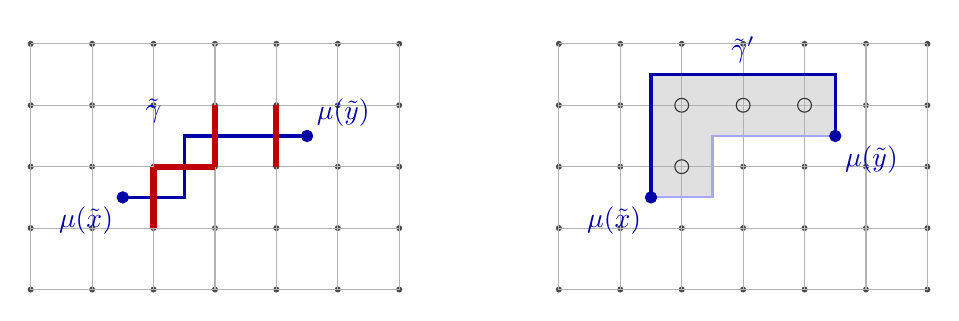
\begin{tikzpicture}[scale=0.78]
% ---- left panel: a disorder line ----
\begin{scope}
  % direct lattice
  \foreach \i in {0,...,6} \foreach \j in {0,...,4}
    \fill[black!70] (\i,\j) circle (1.4pt);
  \foreach \i in {0,...,6} \draw[black!30] (\i,0) -- (\i,4);
  \foreach \j in {0,...,4} \draw[black!30] (0,\j) -- (6,\j);
  % dual path gamma-tilde from (1.5,1.5) to (4.5,2.5)
  \draw[very thick, blue!65!black]
    (1.5,1.5) -- (2.5,1.5) -- (2.5,2.5) -- (3.5,2.5) -- (4.5,2.5);
  % crossed (flipped) bonds
  \draw[line width=2.2pt, red!75!black] (2,1) -- (2,2);
  \draw[line width=2.2pt, red!75!black] (2,2) -- (3,2);
  \draw[line width=2.2pt, red!75!black] (3,2) -- (3,3);
  \draw[line width=2.2pt, red!75!black] (4,2) -- (4,3);
  % endpoints
  \filldraw[blue!65!black] (1.5,1.5) circle (2.6pt) node[below left] {$\mu(\tilde x)$};
  \filldraw[blue!65!black] (4.5,2.5) circle (2.6pt) node[above right] {$\mu(\tilde y)$};
  \node[blue!65!black] at (2.0,2.9) {$\tilde\gamma$};
\end{scope}
% ---- right panel: deformed line and flipped region ----
\begin{scope}[xshift=8.6cm]
  \foreach \i in {0,...,6} \foreach \j in {0,...,4}
    \fill[black!70] (\i,\j) circle (1.4pt);
  % shaded region of flipped sites (between the two paths)
  \fill[black!12] (1.5,1.5) -- (2.5,1.5) -- (2.5,2.5) -- (4.5,2.5)
     -- (4.5,3.5) -- (1.5,3.5) -- cycle;
  \foreach \i in {0,...,6} \draw[black!30] (\i,0) -- (\i,4);
  \foreach \j in {0,...,4} \draw[black!30] (0,\j) -- (6,\j);
  % original path (faint)
  \draw[thick, blue!35]
    (1.5,1.5) -- (2.5,1.5) -- (2.5,2.5) -- (3.5,2.5) -- (4.5,2.5);
  % deformed path
  \draw[very thick, blue!65!black]
    (1.5,1.5) -- (1.5,3.5) -- (4.5,3.5) -- (4.5,2.5);
  % flipped sites in region
  \foreach \pt in {(2,2),(2,3),(3,3),(4,3)}
    \draw[black!80] \pt circle (3.2pt);
  \filldraw[blue!65!black] (1.5,1.5) circle (2.6pt) node[below left] {$\mu(\tilde x)$};
  \filldraw[blue!65!black] (4.5,2.5) circle (2.6pt) node[below right] {$\mu(\tilde y)$};
  \node[blue!65!black] at (3.0,3.9) {$\tilde\gamma'$};
\end{scope}
\end{tikzpicture}
\caption{The disorder line. Left: a dual-lattice path $\tilde\gamma$
(blue) from $\tilde x$ to $\tilde y$; the couplings on the direct bonds
it crosses (heavy red) are flipped, $J \to -J$. Right: deforming the path
to $\tilde\gamma'$ is undone by flipping the spins (circled) in the
enclosed region --- a change of summation variable --- so the correlator
\eqref{eq:mu-def} depends only on the endpoints: the line is topological,
and only its ends, the disorder operators $\mu$, are physical.}
\label{fig:disorder-line}
\end{figure}

Here is the proof, which is one change of variables. Let $\tilde\gamma'$
be another dual path with the same endpoints. The union
$\tilde\gamma \cup \tilde\gamma'$ is a closed dual curve, and a closed
dual curve encloses a definite set $R$ of direct-lattice sites
(Figure~\ref{fig:disorder-line}). Change summation variables in
$Z[\tilde\gamma']$ by flipping every enclosed spin, $s_x \to -s_x$ for $x
\in R$. The bond term $s_x s_y$ changes sign exactly when one endpoint
is inside $R$ and the other outside --- exactly on the bonds crossed by
$\tilde\gamma \cup \tilde\gamma'$. The flip therefore converts the seam
$\tilde\gamma'$ into the seam $\tilde\gamma$, term by term in the sum,
and since relabeling summation variables cannot change the sum,
\begin{equation}
Z[\tilde\gamma'] = Z[\tilde\gamma]:
\label{eq:path-independence}
\end{equation}
the seam is \emph{invisible}; it can be deformed freely so long as its
endpoints stay put. In the language of
Definition~\ref{def:genuine}: the line $\tilde\gamma$ is a
\emph{topological line defect}, and $\mu$ is a \emph{non-genuine}
operator attached to it. The line itself is a seam
across which the configurations are reglued by the $\mathbb{Z}_2$ symmetry $s \to
-s$. It is, in the vocabulary that Part II will make official, the
\emph{symmetry defect} of the $\mathbb{Z}_2$ symmetry --- chapter I.2 found that
Noether charges are topological codimension-one operators
\eqref{eq:topological-charge}; here is the same statement for a discrete
symmetry, with no current anywhere in sight, established by a
change of variables on a lattice. The disorder operator $\mu$ is the
simplest instance of the general slogan: \emph{ends of symmetry defects
are the canonical non-genuine operators}. If the closed curve
$\tilde\gamma\cup\tilde\gamma'$ winds around the periodic lattice rather
than bounding, the flip argument fails --- there is no enclosed region
--- and indeed a seam wrapping a cycle is a physical modification: it
computes the partition function with antiperiodic boundary conditions,
an observable of the \emph{theory on the torus}, distinct from $Z$. The
topology of the line is trivial only up to the topology of spacetime,
a refrain that returns in Section~\ref{sec:defect-hilbert}.

Now compute \eqref{eq:mu-def}, using the low-temperature expansion ---
this is where duality re-enters. In the presence of the seam, the energy
bookkeeping of \eqref{eq:low-T} changes in one place: a crossed bond has
coupling $-J$, so it costs $2J$ when its spins \emph{agree} and is
satisfied when they disagree. Relative to the all-up state, a configuration with
domain-wall curve $\omega$ (on the dual lattice, as before) now has
energy cost $2J$ times the length of the \emph{symmetric difference}
$\omega \,\triangle\, \tilde\gamma$ --- the curve that disagrees either
with the walls or with the seam but not both. Therefore
\begin{equation}
\left\langle \mu(\tilde x) \mu(\tilde y)\right\rangle
= \frac{\sum_{\omega\ \mathrm{closed}} e^{-2J\left|\omega \triangle
\tilde\gamma\right|}}{\sum_{\omega\ \mathrm{closed}} e^{-2J|\omega|}}
= \frac{\sum_{\partial\omega' = \{\tilde x, \tilde y\}}
e^{-2J|\omega'|}}{\sum_{\partial\omega' = \varnothing} e^{-2J|\omega'|}},
\label{eq:mumu-walls}
\end{equation}
where the second equality substitutes $\omega' = \omega \triangle
\tilde\gamma$, which runs over curve configurations with endpoints
$\{\tilde x, \tilde y\}$ as $\omega$ runs over closed ones. Compare
\eqref{eq:high-T-correlator}: the right-hand side of
\eqref{eq:mumu-walls} is precisely the high-temperature representation of
a \emph{spin} two-point function, on the dual lattice, at the coupling
$J^*$ for which $\tanh J^* = e^{-2J}$. We have derived
\begin{equation}
\left\langle \mu(\tilde x)\, \mu(\tilde y) \right\rangle_{J}
= \left\langle s_{\tilde x}\, s_{\tilde y} \right\rangle_{J^*} :
\label{eq:mu-equals-sigma}
\end{equation}
\emph{the disorder operator of the Ising model is the order operator of
its Kramers--Wannier dual}. Equation \eqref{eq:mu-equals-sigma} is exact,
at every coupling and every separation, with no continuum limit and no
criticality assumed. The duality of partition functions
\eqref{eq:kw-coupling} has been upgraded to a duality of operators, and
the upgrade required introducing an extended operator: the dual of a
perfectly ordinary local operator is the endpoint of a line. There is no
way to state Kramers--Wannier as a map of local operators only --- a
first, fully computable demonstration that the extended operators are
not optional.

\begin{eequation}[Order--disorder duality]
\label{eq:kw-box}
\begin{equation*}
\left\langle \mu(\tilde x) \mu(\tilde y) \right\rangle_{J}
= \left\langle s_{\tilde x} s_{\tilde y} \right\rangle_{J^*},
\qquad \sinh 2J \sinh 2J^* = 1 .
\end{equation*}
The endpoint of the topological $\mathbb{Z}_2$ seam at coupling $J$ has exactly
the correlations of the local spin at the dual coupling $J^*$. At the
self-dual point $J = J^* = J_c$, order and disorder correlators become
equal.
\end{eequation}

\begin{exercise}[easy]
\label{exr:1d-disorder}
(The whole construction, in one dimension.) For the periodic Ising chain
of chapter I.1 (Example~\ref{ex:ising-chain}: $N$ sites, weight
$e^{J s_i s_{i+1}}$ per bond, transfer matrix with eigenvalues $\lambda_\pm
= 2\cosh J, 2\sinh J$), the ``dual lattice'' consists of the bond
midpoints, and a disorder pair $\mu(\tilde i)\mu(\tilde j)$ flips the
couplings on the $r$ bonds between them. Show by transfer matrices that
\begin{equation*}
\langle \mu \mu \rangle = \frac{Z[\text{flipped}]}{Z}
\xrightarrow{N\to\infty} (\tanh J)^{r} = \langle s_0 s_r \rangle :
\end{equation*}
in $d = 1$ the disorder correlator coincides with the order correlator at
the \emph{same} coupling. Interpret: the 1d model is its own dual, the
seam endpoints create the domain-wall excitations, and the chain's lack
of a phase transition is the statement that $\sigma$- and $\mu$-type
correlations always decay together.
\hint{Flipping the coupling on a bond replaces its transfer matrix $T =
e^J I + e^{-J}\sigma_x$ by $T' = e^{-J} I + e^{J}\sigma_x = \sigma_x T$
,
so the flipped partition function is a trace of $T$'s with a $\sigma_x$
inserted at each end of the flipped stretch; diagonalize in the
$\ket\pm$ basis where $\sigma_x\ket\pm = \pm\ket\pm$.}
\answ{$Z[\text{flipped}]/Z = (\lambda_+^{N-r}\lambda_-^r +
\lambda_-^{N-r}\lambda_+^r)/(\lambda_+^N + \lambda_-^N) \to
(\lambda_-/\lambda_+)^r = (\tanh J)^r$ --- identical to chapter I.1's
$\langle s_0 s_r\rangle$, computed there by inserting $\sigma_z$'s. The
domain-wall interpretation: $\sigma_x$ inserted in the transfer-matrix
product creates a wall, and $\tanh J$ per step is the wall's propagation
weight.}
\end{exercise}

\subsubsection{What the disorder operator diagnoses}
\label{sec:mu-diagnoses}

The relation \eqref{eq:mu-equals-sigma} converts known facts about the
spin into new physics of the seam, and the conversion is the template for
every ``line operators diagnose phases'' statement in these notes,
including the gauge-theory one of the next section. Read
\eqref{eq:mu-equals-sigma} in each phase.

In the disordered phase $J < J_c$, the dual coupling is supercritical,
$J^* > J_c$, so the dual spin orders:
$\langle s_{\tilde x} s_{\tilde y}\rangle_{J^*} \to (m^*)^2 \neq 0$ at
large separation. Translated: $\langle \mu\mu\rangle$ tends to a nonzero
constant --- the disorder operator \emph{condenses},
$\langle\mu\rangle = m^* \neq 0$, in precisely the phase where the order
operator does not. Physically: $\mu$'s seam reglues configurations by a
spin flip, and in a disordered ensemble, where spins carry no long-range
memory of their sign, regluing costs only a local disturbance near each
endpoint; the line, though arbitrarily long, is free.

In the ordered phase $J > J_c$, the dual spin is disordered and
$\langle\mu\mu\rangle \sim e^{-|\tilde x - \tilde y|/\xi^*}$ decays
exponentially. Physically: in an ordered background the seam is a real
obstruction --- the cheapest configuration in \eqref{eq:mumu-walls} is a
domain wall stretched between the two endpoints, paying tension all along
its length --- and the correlator falls with the \emph{length of the
cheapest wall connecting the insertions}. The exponential decay of a
disorder pair is the two-dimensional shadow of the area law that will
diagnose confinement in Section~\ref{sec:gauge-lines}: there, as here,
the criterion is whether an extended object's cost grows with its size,
and there, as here, the growth happens in the phase where the dual
charge has condensed.

The pair $(\langle\sigma\rangle, \langle\mu\rangle)$ therefore separates
the phase diagram cleanly:
\begin{equation}
\begin{aligned}
J > J_c &: \quad \langle\sigma\rangle \neq 0,\ \ \langle\mu\rangle = 0
&&\text{(ordered; $\mathbb{Z}_2$ broken)},\\
J < J_c &: \quad \langle\sigma\rangle = 0,\ \ \langle\mu\rangle \neq 0
&&\text{(disordered; $\mathbb{Z}_2$ unbroken)},\\
J = J_c &: \quad \langle\sigma\rangle = \langle\mu\rangle = 0,\ \
\text{both correlators power-law}
&&\text{(critical).}
\end{aligned}
\label{eq:phase-table}
\end{equation}
The disordered phase, featureless to every local order parameter, has an
order parameter after all --- an extended one. This is the resolution of
an old embarrassment of the Landau classification (how can a phase with
\emph{no} broken symmetry be distinguished from another such phase?), and
its systematic development --- where the condensing objects are lines and
surfaces and the ``symmetries'' they break are the generalized symmetries
of Part II --- is the generalized Landau paradigm of Part II.8. At the
critical point both expectation values vanish and both two-point
functions obey the same power law,
\begin{equation}
\left\langle \sigma\sigma \right\rangle_{J_c} \sim
\left\langle \mu\mu \right\rangle_{J_c} \sim \frac{1}{|x|^{1/4}},
\qquad \Delta_\sigma = \Delta_\mu = \tfrac18,
\label{eq:critical-sigma-mu}
\end{equation}
the equality of dimensions being forced by self-duality
\eqref{eq:mu-equals-sigma} at $J = J^* = J_c$ (the value $\frac18$ itself
is Onsager-era input, derived three ways in Part III.4). In the continuum
limit at $J_c$, then, the Ising CFT contains two scalar primaries of
dimension $\frac18$: the genuine local operator $\sigma$, and the
non-genuine $\mu$, attached to the topological $\mathbb{Z}_2$ line. They are not
related by any local similarity transformation --- one is mutually local
with everything, the other is not, as we now verify.

\begin{exercise}[medium]
\label{exr:mu-condensate}
(The disorder condensate, to leading order.) Deep in the disordered
phase ($J \to 0$), compute $\langle\mu(\tilde x)\mu(\tilde y)\rangle$
directly from the definition \eqref{eq:mu-def}, by expanding both
$Z[\tilde\gamma]$ and $Z$ to second order in $J$. A naive guess is that
every crossed bond suppresses the ratio, which would make the correlator
decay exponentially in the seam \emph{length} and contradict path
independence. Show instead that each crossed bond contributes
$\frac{\cosh(-J)}{\cosh J} = 1$, and that all corrections organize into
\emph{endpoint} contributions plus terms exponentially small in the
separation, so that
$\langle\mu\mu\rangle \to \langle\mu\rangle^2 \neq 0$. Then check
consistency with duality: $\langle\mu\rangle^2 = (m^*)^2$ with $m^*$ the
spontaneous magnetization at $J^* \to \infty$, which tends to $1$, and
indeed your direct computation gives $\langle\mu\mu\rangle \to 1$ as $J
\to 0$.
\hint{At $J = 0$ exactly, $Z[\tilde\gamma] = Z = 2^N$: flipping
couplings is invisible when spins are uncorrelated, so
$\langle\mu\mu\rangle = 1$ on the nose. Work at small $J$ and watch the
high-temperature graphs of \eqref{eq:high-T}: a graph contributes a sign
$(-1)^{\#(\Gamma \cap \tilde\gamma)}$, and closed graphs cross the seam
an even number of times unless they wind around an endpoint.}
\end{exercise}

\subsubsection{Mutual locality, and a fermion from spins}
\label{sec:mutual-locality-ising}

The operator content assembled so far --- genuine $\sigma$, attached
$\mu$ --- carries one more computable structure: the two are mutually
non-local, and the failure is a clean $\mathbb{Z}_2$ monodromy. Consider a
correlator with both insertions,
$\langle s_z\, \mu(\tilde x)\mu(\tilde y) \rangle$, defined by
\eqref{eq:flipped-Z} with a spin inserted. The path-independence
argument \eqref{eq:path-independence} acquires an exception: deforming
$\tilde\gamma$ across the site $z$ flips the summation variable $s_z$,
which now sits \emph{in the correlator}, not only in the weight. The
correlator with the deformed seam equals \emph{minus} the original:
\begin{equation}
\left\langle s_z\, \mu\mu \right\rangle_{\tilde\gamma'}
= - \left\langle s_z\, \mu\mu \right\rangle_{\tilde\gamma}
\qquad \text{when } \tilde\gamma' - \tilde\gamma \text{ sweeps across } z.
\label{eq:mutual-sign}
\end{equation}
Equivalently: transporting $\sigma$ around one endpoint $\mu$ along a
closed loop --- which forces the seam to be swept across $\sigma$ once
--- returns the correlator with a factor $(-1)$. The pair
$(\sigma, \mu)$ is \vocab{mutually semi-local} with monodromy $-1$. This
is the lattice prototype of the linking phases that govern which line
operators may coexist in gauge theory
(Section~\ref{sec:dirac-pairing}); there as here, the phase is
computed by an entirely kinematic argument --- no dynamics, only the
bookkeeping of what crosses what.

Kadanoff and Ceva noticed what the monodromy is good for. Place the two
mutually semi-local operators at nearest-neighbor positions --- a spin
$s_x$ and an adjacent disorder operator $\mu(\tilde x)$ --- and call the
composite
\begin{equation}
\psi(x, \tilde x) \sim s_x\, \mu(\tilde x).
\label{eq:kc-fermion}
\end{equation}
Rotate the plane by $2\pi$ about the composite. The seam attached to
$\mu$ is dragged once completely around, and in the course of the
rotation it sweeps across the partner spin $s_x$ exactly once: by
\eqref{eq:mutual-sign}, the configuration returns to itself with a
factor $(-1)$. An operator that changes sign under a $2\pi$ rotation has
half-integer spin. The Ising model --- commuting variables, not a
Grassmann number in sight --- contains a \emph{fermion}, assembled from
an order and a disorder operator, with the minus sign of Fermi
statistics supplied by the topology of the attached line. At the
critical point the composite becomes a conformal field of dimensions
$(h, \bar h) = (\frac12, 0)$ (and its conjugate $(0, \frac12)$), with
\begin{equation}
\left\langle \psi(x) \psi(0) \right\rangle \sim \frac{1}{x},
\label{eq:kc-correlator}
\end{equation}
the free-fermion correlator: the continuum limit of the critical Ising
model is, in this precise operator-by-operator sense, a theory of free
Majorana fermions.\footnote{Kadanoff--Ceva, op.\ cit., established
\eqref{eq:kc-correlator} on the lattice. The statement that the
$\sigma\mu$ composite has spin $\frac12$, argued here by monodromy, is
visible in the exact lattice correlators; the free-fermion description
is completed by the Onsager/Schultz--Mattis--Lieb solution and is
derived in the continuum in Part III.4, with the global structure ---
in what sense the Ising CFT and the Majorana CFT are and are not the
same theory --- in Parts II and VIII (Seiberg--Shao \arxiv{2307.02534}
is the careful modern treatment).} Fermionization, bosonization, the
Jordan--Wigner transformation --- the entire technology by which
two-dimensional physics trades spins for fermions --- is the systematic
exploitation of \eqref{eq:kc-fermion}, and the reader who tracks where
the Jordan--Wigner ``string'' goes will find it is exactly the disorder
seam (Exercise~\ref{exr:quantum-kw}).

\begin{iidea}[Extended operators are made, and make, new physics]
\label{idea:mu-payoff}
The disorder line was constructed from the symmetry of the theory (a
$\mathbb{Z}_2$ seam), proved topological by a change of variables, and found to
carry, at its ends, operators that (i) serve as the order parameter of
the symmetry-\emph{unbroken} phase, (ii) realize the dual model's local
operators, and (iii) combine with local operators into fields of new
spin and statistics. None of this data is visible in, or derivable
from, the correlators of genuine local operators alone --- yet all of
it is exact, lattice-computable physics. ``The definition of a theory
includes its extended operators'' is not a definition being defended;
it is a description of what the Ising model was found to contain.
\end{iidea}

The construction generalizes in every direction, and the
generalizations are best signposted now, while the mechanism is fresh.
For a $\mathbb{Z}_N$ or $U(1)$ symmetry, the seam reglues by a symmetry element
$g$ and the endpoint operators carry a $g$-dependent monodromy ---
disorder operators exist for every global symmetry of every lattice
model. In higher dimensions $d$, the seam is a codimension-one sheet
$\tilde\Sigma_{d-1}$ of flipped bonds, its boundary a codimension-two
disorder operator: in the 3d Ising model the disorder operator is a
\emph{line} (the boundary of a flipped-bond membrane), whose
condensation--versus--tension dichotomy again diagnoses the phases, and
whose gauge-theory counterpart is the 't~Hooft line met momentarily.
And when the symmetry being reglued is a \emph{gauge} redundancy rather
than a global symmetry, the seam itself becomes invisible in a stronger
sense but its possible boundaries reorganize: that story is the next
section's. The single lattice mechanism --- flip couplings across a
hypersurface, watch the boundary --- underlies all of it.

\begin{exercise}[medium]
\label{exr:quantum-kw}
(Kramers--Wannier and the disorder operator in the quantum chain.) The
transfer-matrix limit of the 2d Ising model (chapter I.1's
Example~\ref{ex:ising-chain} logic, run with a spatial dimension kept)
is the transverse-field Ising chain: $N$ sites, Pauli operators $X_j,
Z_j$, Hamiltonian
\begin{equation*}
H = -g\sum_{j=1}^{N} X_j - \sum_{j=1}^{N} Z_j Z_{j+1},
\end{equation*}
periodic identification $N + 1 \equiv 1$; the ordered phase is $g < 1$,
the disordered $g > 1$, the critical point $g = 1$, and the $\mathbb{Z}_2$
symmetry is $\eta = \prod_j X_j$. (a) Define dual-site variables
\begin{equation*}
\tilde Z_{j+\frac12} = \prod_{i \le j} X_i ,
\qquad
\tilde X_{j+\frac12} = Z_j Z_{j+1},
\end{equation*}
and check they obey the Pauli algebra on the dual sites (commuting at
different sites, anticommuting on-site). (b) Show $X_j = \tilde
Z_{j-\frac12}\tilde Z_{j+\frac12}$ and hence $H(g) = g \tilde H(1/g)$
with $\tilde H$ the same Hamiltonian in dual variables: Kramers--Wannier
as an exact rewriting, self-dual at $g = 1$. (c) Identify $\mu_{j+\frac12}
= \tilde Z_{j+\frac12}$: a half-infinite \emph{string} of spin flips ---
the quantum-chain incarnation of the seam, manifestly attached to a line
(the string), manifestly the order parameter of the $g > 1$ phase (where
$X_j \approx +1$ and the string averages to a nonzero value). (d) On the
periodic chain, show the string cannot close consistently: a single
$\mu$ is not an operator on the untwisted Hilbert space, only $\mu$
pairs are --- and a single $\mu$ instead lives in the Hilbert space
twisted by $\eta$ (Section~\ref{sec:defect-hilbert}). (e) Combine with a
Jordan--Wigner transformation to exhibit the Kadanoff--Ceva fermion as
$\psi_j \sim Z_j \prod_{i<j} X_i$, and verify
$\{\psi_i, \psi_j\} \propto \delta_{ij}$: the string makes commuting
variables anticommute.
\hint{For (d): formally, $\prod_{i\le N} X_i = \eta$, so the
``closed-up'' string is the symmetry operator itself, not an endpoint
operator; the obstruction to ending it is the $\mathbb{Z}_2$ charge it would
leak. Each part is a short computation; the content is in reading them.}
\end{exercise}

\begin{ppreview}[The seam at the self-dual point: a non-invertible line]
At $J = J_c$ the model equals its dual, so Kramers--Wannier becomes a
\emph{symmetry of one theory} --- and, since it maps the genuine
$\sigma$ to the attached $\mu$, it cannot be implemented by any unitary
operator. It is implemented by a topological line $\mathcal D$ with the
fusion rule $\mathcal D \times \mathcal D = 1 + \eta$: a
\vocab{non-invertible symmetry}, the first ever identified, and on the
lattice an explicit $2^N \times 2^N$ matrix commuting with the critical
chain Hamiltonian. Part II.5 builds this properly (Shao
\arxiv{2308.00747}, \S3, is the source); it is mentioned here because
the reader now owns every ingredient: the $\eta$ seam, the duality, and
the order--disorder exchange.
\end{ppreview}

% =====================================================================
\subsection{Lines in gauge theory: the spectrum is part of the definition}
\label{sec:gauge-lines}

Gauge theory in four dimensions is where the chapter's thesis was
sharpened into a precise statement, and the logic tracks the Ising
construction step for step: an order-type line (Wilson), a disorder-type
line ('t~Hooft), a mutual-locality constraint (Dirac), and the discovery
that consistent maximal choices of lines are \emph{plural} --- distinct
theories, agreeing on all local correlators, distinguished only between
the lines. The section develops each step in turn. Throughout, ``gauge
theory'' means the quantum theory built from a gauge \emph{algebra}
$\lie g$ together with whatever additional global data the analysis turns
out to demand; part of the point is to watch that demand emerge.

\subsubsection{The Wilson line}
\label{sec:wilson-line}

The Wilson line answers a physical question: what does the gauge theory
do to an external charge? Take Maxwell theory first --- a $U(1)$ gauge
field with Euclidean action $S = \frac{1}{4e^2}\int d^4x\,
F_{\mu\nu}F_{\mu\nu}$ --- and introduce a probe particle of charge $q
\in \ints$, infinitely heavy so that it has no dynamics of its own: it
simply sits on a prescribed worldline $C$. The coupling of a charge to
the gauge field is $q\int_C A$, so integrating out the probe leaves
behind the insertion
\begin{equation}
W_q(C) = \exp\left( i q \oint_C A_\mu\, dx^\mu \right),
\label{eq:wilson-u1}
\end{equation}
the \vocab{Wilson line} of charge $q$. For a nonabelian algebra the
exponential must be path-ordered and traced in a chosen representation
$R$,
\begin{equation}
W_R(C) = \tr_R\, \mathrm{P} \exp\left( i \oint_C A \right),
\label{eq:wilson-nonabelian}
\end{equation}
because the probe now carries internal color states that the gauge field
rotates as it moves; the trace sums over the probe's internal states,
and gauge invariance of the closed loop follows from cyclicity. The
label of a Wilson line is therefore a representation, and which
representations are allowed is exactly the question this section
builds toward.

Equation \eqref{eq:wilson-nonabelian} is the order-type construction
\eqref{eq:order-defect} in gauge-theory clothing --- a coupling
integrated along the defect --- and, like the Ising impurity, it serves
as a probe of the vacuum. The diagnostic works as follows. Take
$C$ to be a rectangle: a charge--anticharge pair created at some time,
held at separation $R$ for a Euclidean time $T \gg R$, then annihilated.
The path integral with this insertion computes the amplitude for the
static pair to persist, so
\begin{equation}
\left\langle W(C_{R \times T}) \right\rangle \sim e^{- T\, V(R)},
\qquad T \to \infty,
\label{eq:wilson-potential}
\end{equation}
with $V(R)$ the energy of the static pair: the interquark potential,
extracted from a line operator's expectation value. The two
characteristic large-loop behaviors,
\begin{equation}
\left\langle W(C) \right\rangle \sim
\begin{cases}
e^{-c\, \mathrm{Perimeter}(C)} & \text{\vocab{perimeter law}: } V(R) \to
\text{const}, \text{ liberated charges},\\[2pt]
e^{-\varsigma\, \mathrm{Area}(C)} & \text{\vocab{area law}: } V(R) =
\varsigma R, \text{ confinement, string tension } \varsigma,
\end{cases}
\label{eq:area-perimeter}
\end{equation}
distinguish phases of the gauge theory --- Wilson's criterion. A
perimeter-law contribution is always present (it is the probe's
self-energy, the divergence met in Example~\ref{ex:static-impurity},
removed by a worldline counterterm), so the content of
\eqref{eq:area-perimeter} is whether, after that subtraction, the loop
feels its area. The parallel with the Ising disorder pair is exact: an
extended object whose cost grows with its extent (wall tension there,
string tension here) signals one phase; an extended object that gets
free of its extent signals the other. Which object does which depends on
the phase, and having \emph{both} an order line and a disorder line in
hand is what makes the diagnostics complete --- the burden of
Section~\ref{sec:thooft-line}.

\begin{eexample}[The Wilson loop in free Maxwell theory]
\label{ex:maxwell-wilson}
The one gauge theory where \eqref{eq:wilson-potential} can be evaluated
from start to finish is the free Maxwell field, and we do it once in
full, because the evaluation separates what is special to free fields
from what is structural. The theory is Gaussian, so
\begin{equation}
\left\langle W_q(C) \right\rangle
= \exp\left( -\frac{q^2}{2} \oint_C \oint_C dx^\mu dy^\nu
\left\langle A_\mu(x) A_\nu(y) \right\rangle \right),
\label{eq:maxwell-w-gaussian}
\end{equation}
with the photon propagator in Feynman gauge $\langle A_\mu(x)
A_\nu(0)\rangle = \frac{e^2 \delta_{\mu\nu}}{4\pi^2 x^2}$ (the
gauge-dependent pieces integrate to zero around closed loops). Evaluate
on the $R \times T$ rectangle, $T \gg R$. The double line integral
splits into self-pairings of each side and cross-pairings. The
self-pairing of each long side is the divergent self-energy ---
$\frac{e^2 q^2}{4\pi^2}\, T \int \frac{ds}{s^2}$, linear in $T$ with a
short-distance divergent coefficient, the worldline mass counterterm
again. The physics is in the cross-pairing of the two long sides, which
are traversed in opposite directions (relative minus sign):
\begin{equation}
-2 \times \frac{e^2 q^2}{2}
\int_0^T dt \int_0^T dt'\,
\frac{(-1)}{4\pi^2\left[(t - t')^2 + R^2\right]}
\xrightarrow{T \gg R}
+ \frac{e^2 q^2\, T}{4\pi^2} \int_{-\infty}^{\infty}
\frac{ds}{s^2 + R^2}
= \frac{e^2 q^2\, T}{4\pi R}.
\end{equation}
Assembling via \eqref{eq:wilson-potential} (and absorbing the
self-energies into the counterterm),
\begin{equation}
V(R) = -\frac{e^2 q^2}{4\pi R}:
\label{eq:coulomb-from-loop}
\end{equation}
the Coulomb attraction of a static pair, recovered as the area-free,
perimeter-renormalized content of a line operator's expectation value.
Free Maxwell theory is in the perimeter-law class --- charges can be
separated at finite cost --- as expected for a theory of free photons.
The reader should note which features of the computation were specific
to free fields (the Gaussian closing of the exponential) and which were
not (the worldline counterterm; the extraction of $V(R)$; the
perimeter/area alternative): in strongly coupled Yang--Mills the former
fails utterly while the latter organizes the numerical and theoretical
study of confinement to this day.
\end{eexample}

\begin{exercise}[medium]
\label{exr:cusp}
(Cusps.) The rectangle has four corners, and the cross-pairings of
adjacent sides produce, besides the finite potential, a logarithmic
divergence localized at each corner. Extract it: show that two straight
segments meeting at an angle $\theta$ contribute to $-\ln\langle W
\rangle$ a term $\frac{e^2 q^2}{4\pi^2}\,\Gamma_{\rm cusp}(\theta) \ln
(L/a)$ with $a$ a short-distance cutoff, and compute
$\Gamma_{\rm cusp}$ at this (lowest) order. Smooth loops have no such
divergence: the renormalization of a line operator depends on the
\emph{geometry} of its support --- length divergences always, angle
divergences at cusps. (The cusp anomalous dimension became a central
object of gauge-theory integrability and of the modern amplitudes
program, Part IX.)
\hint{Parametrize the two segments from the common corner and use the
same propagator; the $\ln$ arises from the region where both points
approach the corner. $\Gamma_{\rm cusp}(\theta) \propto \theta\cot\theta
- 1$ in Euclidean signature at this order.}
\end{exercise}

\subsubsection{The 't~Hooft line, and mutual locality}
\label{sec:thooft-line}
\label{sec:dirac-pairing}

The Wilson line used only the order-type construction, and the Ising
analysis instructs us to seek its disorder partner. In Maxwell theory the
recipe of Section~\ref{sec:disorder-type} applies verbatim: excise a
line $L$ from spacetime and sum over gauge fields with prescribed
singular behavior around it --- prescribed flux through the linking
two-sphere,
\begin{equation}
\int_{S^2_{\mathrm{link}}} F = 2\pi m, \qquad m \in \ints :
\label{eq:thooft-def}
\end{equation}
the \vocab{'t~Hooft line} of magnetic charge $m$, the worldline of an
infinitely heavy magnetic monopole that the theory does not contain as a
dynamical particle.\footnote{G.~'t~Hooft, \emph{On the phase transition
towards permanent quark confinement}, Nucl.\ Phys.\ B \textbf{138}
(1978) 1, which introduced both the operator and the order/disorder
classification of gauge-theory phases used in this section. The
quantization of $m$ in \eqref{eq:thooft-def} is Dirac's: $F$ is the
curvature of a $U(1)$ bundle on $S^2_{\rm link}$, and its flux is
$2\pi$ times the bundle's Chern number.} No term is added to the
action; the configuration space is enlarged to include monopole sectors
around $L$. The construction is the vortex defect
\eqref{eq:vortex-defect} with the winding of a scalar replaced by the
flux of a gauge field, and the codimension adjusted to match: in $d = 4$
a line has codimension three, its linking sphere is the
\emph{two}-sphere, and flux through $S^2$ is therefore the data that
can be prescribed.

Wilson and 't~Hooft lines are mutually constrained, and the constraint
is the gauge-theory version of the Ising monodromy
\eqref{eq:mutual-sign}. Transport a Wilson line of charge $q$ around a
closed loop $\gamma$ that links the 't~Hooft line of charge $m$ once.
The Wilson insertion is $e^{iq\oint_\gamma A}$, and as $\gamma$ is swept
around the monopole worldline it spans a closed surface through which
the flux is \eqref{eq:thooft-def}; the holonomy changes by
\begin{equation}
\exp\left( i q \int_{S^2} F \right) = e^{2\pi i\, q m}.
\label{eq:linking-phase}
\end{equation}
For integer $q$ and $m$ this phase is $1$ and the two insertions are
mutually local: Maxwell theory with charges in $\ints$ admits both
families as genuine lines. But the phase \eqref{eq:linking-phase} is the
general currency, and it becomes a nontrivial constraint the moment fractional pairings
appear --- as they do for every nonabelian algebra with a nontrivial
center. For dyonic lines carrying both charges, $(q, m)$ and $(q', m')$,
the same sweep produces the \vocab{Dirac--Schwinger--Zwanziger pairing}
\begin{equation}
\left\langle (q,m), (q',m') \right\rangle
= q\, m' - m\, q' ,
\label{eq:dsz}
\end{equation}
and single-valuedness of correlators demands that the pairing be an
integer (in the units where \eqref{eq:linking-phase} is $e^{2\pi i (q m'
- m q')}$, an element of $\ints$) for every pair of lines the theory
contains. Mutual locality is not automatic; it is a constraint on the
\emph{set} of lines, and sets obeying it are in general far from unique.

\subsubsection{$SU(2)$ versus $SO(3)$: one algebra, three theories}
\label{sec:su2-so3}

Now run the constraint in the simplest nonabelian setting, following
Aharony--Seiberg--Tachikawa.\footnote{\arxiv{1305.0318}, \S1, whose
presentation this subsection compresses; the general-group analysis is
their \S\S2--6. The underlying observation that the line spectrum
distinguishes gauge groups goes back to
Kapustin \texttt{hep-th/0501015} and is implicit in 't~Hooft's
classification.} Take pure Yang--Mills theory with algebra $\lie{su}(2)$
and no matter. Local operators --- gauge-invariant polynomials in the
field strength and its derivatives --- are blind to the global form of
the gauge group: their correlators on $\reals^4$ are identical whether
``the gauge group'' is taken to be $SU(2)$ or $SO(3) = SU(2)/\ints_2$.
If the theory were its local correlators, the choice would be a
convention. It is not, and the lines show it.

Charge labels: electric charge under the center of $SU(2)$ is a weight
modulo roots, $z_e \in \ints_2$ --- integer spin representations have
$z_e = 0$, half-integer spin (the fundamental) $z_e = 1$ --- and
magnetic charge likewise, $z_m \in \ints_2$, by running
\eqref{eq:thooft-def} with the dual group's weights. A line class is a
pair $(z_e, z_m) \in \ints_2 \times \ints_2$, four classes in all, and
the pairing \eqref{eq:dsz} reduces mod 2:
\begin{equation}
\left\langle (z_e, z_m), (z'_e, z'_m)\right\rangle
= z_e z'_m - z_m z'_e \mod 2 .
\label{eq:z2-pairing}
\end{equation}
A consistent theory must pick a set of classes that (i) is closed under
fusion (bringing two lines together gives a line, so the set is a
subgroup), (ii) is mutually local --- the pairing
\eqref{eq:z2-pairing} vanishes on the set --- and (iii) is
\emph{maximal}: any class mutually local with everything in the set is
in the set. Maximality is the statement that there is no obstruction to
including a consistent line, so excluding it would amount to declaring
extra structure that is not there; relaxing it leads not to new theories
but to incomplete descriptions of these same ones (the systematic
account of why, via one-form symmetries and gauging, is Part II.4's).
The subgroup $\{(0,0)\}$ alone fails (iii), since everything pairs to
zero with it. The enumeration is then a one-line exercise in
$\ints_2\times\ints_2$: the maximal mutually local subgroups are exactly
the three order-two subgroups,
\begin{equation}
\begin{aligned}
\{(0,0), (1,0)\} &: \quad SU(2) \quad
&&\text{Wilson line in the fundamental; no fundamental 't Hooft line},\\
\{(0,0), (0,1)\} &: \quad SO(3)_+ \quad
&&\text{fundamental 't Hooft line; no fundamental Wilson line},\\
\{(0,0), (1,1)\} &: \quad SO(3)_- \quad
&&\text{only the dyonic line carries nontrivial charge},
\end{aligned}
\label{eq:three-theories}
\end{equation}
--- \emph{three} distinct quantum field theories built on the single
algebra $\lie{su}(2)$, sharing every local correlator on $\reals^4$,
distinguished by which extended operators exist
(Figure~\ref{fig:line-lattices}). The names record that the Wilson lines
of $SU(2)$ are those of the simply connected group (all
representations), while both $SO(3)$ theories admit only integer-spin
Wilson lines, differing from each other in their magnetic sector. This
is the resolution --- in the affirmative, with an exact count --- of
chapter I.1's Exercise~\ref{exr:two-theories-same-correlators}.

\begin{figure}[t]
\centering
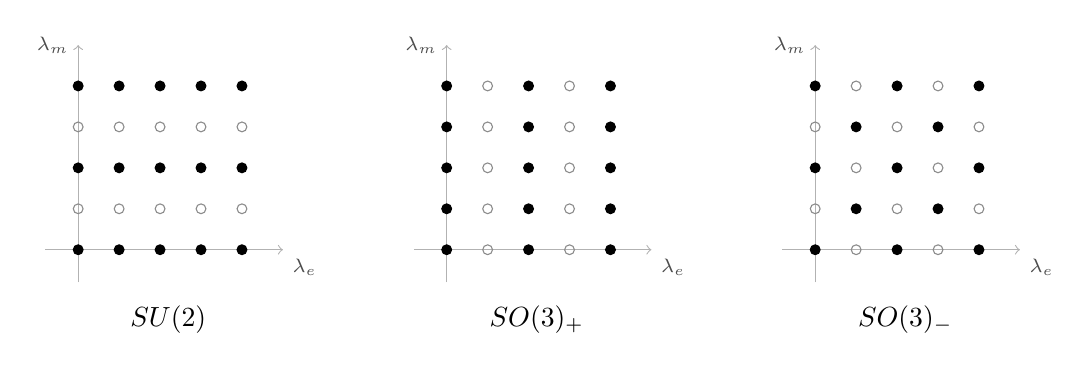
\begin{tikzpicture}[scale=0.52]
\foreach \panel/\name in {0/{SU(2)}, 9/{SO(3)_+}, 18/{SO(3)_-}}{
\begin{scope}[xshift=\panel cm]
  % axes
  \draw[->, gray!60] (-0.8,0) -- (5.0,0) node[below right, black!70] {\scriptsize $\lambda_e$};
  \draw[->, gray!60] (0,-0.8) -- (0,5.0) node[left, black!70] {\scriptsize $\lambda_m$};
  \node at (2.2,-1.7) {$\name$};
\end{scope}
}
% SU(2): lambda_e any integer, lambda_m even
\begin{scope}
\foreach \i in {0,...,4} \foreach \j in {0,2,4}
  \filldraw[black] (\i,\j) circle (3.4pt);
\foreach \i in {0,...,4} \foreach \j in {1,3}
  \draw[black!45] (\i,\j) circle (3.4pt);
\end{scope}
% SO(3)+: lambda_e even, lambda_m any
\begin{scope}[xshift=9cm]
\foreach \i in {0,2,4} \foreach \j in {0,...,4}
  \filldraw[black] (\i,\j) circle (3.4pt);
\foreach \i in {1,3} \foreach \j in {0,...,4}
  \draw[black!45] (\i,\j) circle (3.4pt);
\end{scope}
% SO(3)-: lambda_e + lambda_m even
\begin{scope}[xshift=18cm]
\foreach \i in {0,...,4} \foreach \j in {0,...,4}
{
  \pgfmathparse{mod(\i+\j,2)}
  \ifdim\pgfmathresult pt=0pt
    \filldraw[black] (\i,\j) circle (3.4pt);
  \else
    \draw[black!45] (\i,\j) circle (3.4pt);
  \fi
}
\end{scope}
\end{tikzpicture}
\caption{The line operators of the three theories with gauge algebra
$\lie{su}(2)$, after Aharony--Seiberg--Tachikawa. Each panel shows the
electric--magnetic charge lattice $(\lambda_e, \lambda_m)$; filled dots
are the lines the theory contains, open circles those it excludes. All
three sets are closed under fusion, mutually local under the pairing
\eqref{eq:dsz}, and maximal --- and no two are the same set.}
\label{fig:line-lattices}
\end{figure}

That the three theories differ is so far a statement about which
correlators exist. The differences reach physics with no visible
connection to global structure, along three channels that the rest of
these notes will use repeatedly: phase diagnostics, the periodicity of
$\theta$, and compactification.

\emph{Phase diagnostics.} In a confining $SU(2)$ vacuum the fundamental
Wilson line shows an area law. In $SO(3)_+$ there \emph{is} no
fundamental Wilson line whose area law could be checked: the available
diagnostics are the 't~Hooft line and the dyon, and which of them shows
perimeter law distinguishes vacua --- e.g.\ the two vacua of
$\mathcal{N}=1$ supersymmetric $\lie{su}(2)$ theory, exchanged by
$\theta \to \theta + 2\pi$, are distinguished in $SO(3)_\pm$ by which
line condenses, while in $SU(2)$ they look alike to every line
\arxiv{1305.0318}. Phase classification is relative to the
theory's line content: ``confining'' is not a property of a gauge
algebra but of a theory, tested by the lines that theory possesses.

\emph{The range of $\theta$.} The $\theta$-angle weights instanton
sectors by $e^{i\theta\,\ell}$, and in $SU(2)$ the instanton number
$\ell$ is an integer, making $\theta$ $2\pi$-periodic. In the $SO(3)$
theories there are gauge bundles with $\ell \in \frac12\ints$ (on spin
manifolds), so naively $\theta$ has period $4\pi$ --- but the
Witten effect intervenes: shifting $\theta$ by $2\pi$ shifts the
electric charge of every magnetic line by its magnetic charge,
\begin{equation}
\theta \to \theta + 2\pi: \qquad (\lambda_e, \lambda_m)
\longrightarrow (\lambda_e + \lambda_m,\ \lambda_m),
\label{eq:witten-effect}
\end{equation}
which maps the set $SO(3)_+$ into the set $SO(3)_-$ and back: the two
$SO(3)$ theories are exchanged, not preserved, by a $2\pi$ shift, and
each is $4\pi$-periodic on its own.\footnote{The Witten effect ---
E.~Witten, \emph{Dyons of charge $e\theta/2\pi$}, Phys.\ Lett.\ B
\textbf{86} (1979) 283 --- states that in a $\theta$-vacuum a monopole
of magnetic charge $m$ carries electric charge $q = n + \theta m/2\pi$:
the $\theta$-term, evaluated on a monopole background, acts as an
electric source. Part V.3 derives it; here we use only the bookkeeping
consequence \eqref{eq:witten-effect}.} The periodicity of a coupling
constant --- local-physics data, one would have said --- is set by the
line spectrum.

\emph{Compactification.} Put the theories on $\reals^3 \times S^1$. A
line wrapping the $S^1$ becomes, from the three-dimensional viewpoint, a
\emph{local} operator, so theories differing in their lines differ in
their 3d local operator content --- and at that point not even local
correlators agree anymore. The differences are quantitative and
dramatic: the supersymmetric Witten index (the counting of vacua on a
torus) of $\mathcal{N}=1$ $\lie{su}(2)$ theory differs between $SU(2)$
and the $SO(3)_\pm$ theories \arxiv{1305.0318}. Two theories
indistinguishable by local experiments in infinite flat space are
distinguished by local experiments in a periodic box. For a subject ---
lattice gauge theory, for instance --- that lives in periodic boxes,
the global form is not philosophy.

\begin{iidea}[The line spectrum is part of the definition]
\label{idea:lines-define}
Specifying a gauge theory requires specifying its gauge algebra
\emph{and} its set of line operators --- a maximal mutually local
sublattice of electric--magnetic charges. Distinct maximal choices are
distinct theories: identical on local correlators in $\reals^d$, they
differ in phase diagnostics, in the periodicity of parameters, and in
their physics upon compactification. What was true for the Ising model
(the dual operator lives at the end of a line the local data never
sees) is true for Yang--Mills, with ``which lines exist'' promoted from
a curiosity to a defining datum. Reading between the lines is reading
the definition.
\end{iidea}

\begin{exercise}[classic]
\label{exr:maximal-lattices}
(The enumeration, and its $SU(N)$ generalization.) (a) Verify that
\eqref{eq:three-theories} lists \emph{all} subgroups of $\ints_2 \times
\ints_2$ that are isotropic for the pairing \eqref{eq:z2-pairing} and
maximal, and that maximality is doing work: exhibit a mutually local set
that is consistent but incomplete, and the lines that complete it. (b)
For algebra $\lie{su}(N)$ with $N$ prime, the classes live in $\ints_N
\times \ints_N$ with pairing $z_e z'_m - z_m z'_e \bmod N$. Show the
maximal isotropic subgroups are: the electric one $\{(z_e, 0)\}$
(theory $SU(N)$), and the $N$ subgroups generated by $(k, 1)$ for $k =
0, \dots, N-1$ (theories $(SU(N)/\ints_N)_k$, permuted cyclically by
$\theta \to \theta + 2\pi$) --- $N + 1$ theories per algebra, more than
the two global forms of the group. (c) For non-prime $N$ there are
intermediate quotients and additional discrete labels; count the
theories for $N = 4$.
\hint{For (b): an isotropic subgroup of order $N$ (the maximal order,
by a counting argument mirroring Lagrangian subspaces of a symplectic
form) either contains $(1,0)$-type elements only, or contains an
element with $z_m \neq 0$, which for prime $N$ generates everything of
the form $(kz, z)$. For (c): $SU(4)$, $SU(4)/\ints_2$ with two discrete
$\theta$-like choices, $SU(4)/\ints_4$ with four --- see
\arxiv{1305.0318}, \S6, to check your count.}
\answ{(a) $\{(0,0)\}$ and any single nontrivial class form consistent
but non-maximal sets; each completes uniquely to one of the three. (b)
Isotropy of $\langle(k,1),(k',1)\rangle = k - k' \bmod N$ forces a
single generator; $N+1$ in all. (c) Seven: $1 + 2 + 4$.}
\end{exercise}

\begin{exercise}[medium]
\label{exr:wrapped-lines}
(Wrapped lines as local order parameters.) On $\reals^3 \times
S^1_\beta$, the wrapped fundamental Wilson line of $SU(2)$ --- the
\vocab{Polyakov loop} $P(\mathbf{x}) = \tr\,\mathrm{P}
\exp(i\oint_{S^1} A)$ --- is a genuine local operator of the 3d theory.
(a) Interpreting $S^1_\beta$ as thermal time (chapter I.2's
Exercise~\ref{exr:kms}), show that $\langle P(\mathbf{x})\rangle =
e^{-\beta F_q}$ with $F_q$ the free-energy cost of a single static
quark, so that $\langle P \rangle = 0$ diagnoses confinement and
$\langle P\rangle \neq 0$ deconfinement at temperature $1/\beta$. (b)
Identify the symmetry of the thermal $SU(2)$ theory that $P$ is charged
under --- the center symmetry acting by a $\ints_2$-valued aperiodic
gauge transformation around the circle --- and recast (a) as an
ordinary Landau symmetry-breaking statement \emph{for the wrapped
line}: deconfinement is the spontaneous breaking of center symmetry,
with $P$ its local order parameter. (c) Explain why the $SO(3)_+$
theory, which lacks the fundamental Wilson line, lacks this symmetry
and this order parameter --- the thermal phase structure must be probed
differently, e.g.\ by the wrapped 't~Hooft line. (The symmetry of (b)
is a one-form symmetry in four-dimensional disguise; Part II.4 will
say this properly, and Part V.2 uses it.)
\hint{(a) is the standard thermal interpretation of a static source:
the wrapped line inserts $e^{-\beta H}$-evolution with one infinitely
heavy charge added. (b) The aperiodic transformation multiplies $P$ by
$-1$ but preserves the action and all local operators.}
\end{exercise}

\begin{nnote}
The scope of these statements has two edges that should be marked.
First, this section's lines were \emph{probe}
operators in theories whose dynamical fields are blind to the center;
dynamical fundamental matter (as in QCD) makes the fundamental Wilson
line screenable and breaks the area/perimeter dichotomy --- phase
diagnostics in such theories need the finer tools of Part II (in QCD
proper, strictly speaking, only crossovers and symmetries remain).
Second, the count \eqref{eq:three-theories} is for $\reals^4$ or $S^4$;
on manifolds with more topology the same theories require still more
data (how to sum the $SO(3)$ bundles, the discrete $\theta$-like
parameters of \arxiv{1305.0318} \S\S3, 6), foreshadowing the general
principle of chapter I.4 that a theory is an assignment to \emph{all}
backgrounds at once.
\end{nnote}

The chapter's first two installments --- Ising and Yang--Mills --- carry
the same moral with different machinery, and it is the machinery overlap
that should be memorized: a disorder-type extended operator, a
topological line/surface implementing a symmetry, a monodromy pairing
constraining coexistence, condensation-versus-tension as the phase
diagnostic. Surface operators in four dimensions (the boundaries of
flipped-coupling membranes; Gukov--Witten operators
\texttt{hep-th/0612073} in gauge theory), vortex lines in
three-dimensional scalar theories, and the higher-form generalizations
all run on these rails; Part II turns the rails into the subject.


% =====================================================================
\subsection{Defects as probes: the kinematics of defect CFT}
\label{sec:defect-cft}

So far the chapter has treated extended operators as things to
\emph{define} and to \emph{count}. This section treats them as things to
\emph{measure with}, in the setting where measurement is sharpest: a
conformal field theory hosting a scale-invariant defect. The motivation
is the same as for studying CFTs at all. Just as a generic theory is an
RG flow between fixed points (chapter I.1), a generic \emph{defect} in a
critical system --- an impurity, a boundary, a wall --- flows, as it is
viewed from farther and farther away, to a scale-invariant defect in the
CFT, and the fixed-point data organizes everything universal about the
impurity. The Kondo problem is the classic instance: the screening of a
magnetic impurity by conduction electrons is, in modern language, a
defect RG flow between two defect fixed points of a free-fermion bulk.
What follows is the kinematics of such fixed points: which correlators
are fixed by symmetry, and which numbers --- the \vocab{defect CFT
data} --- a solution of the defect must supply.\footnote{The systematic
treatment in general dimension and codimension is
Bill\`o--Gon\c{c}alves--Lauria--Meineri \arxiv{1601.02883}, which this
section follows; boundaries were done first, by Cardy in 2d (Nucl.\
Phys.\ B \textbf{240} (1984) 514) and by McAvity--Osborn in general $d$
(\texttt{cond-mat/9505127}). Northe's lectures \arxiv{2411.03381},
\S\S7--8, are the gentlest systematic entry.}

\subsubsection{Conformal defects and their one-point functions}

A flat $p$-dimensional defect $\mathcal{D}$ in $\reals^d$ breaks the
conformal group, and the definition of a conformal defect is fixed by
asking how much of it can survive: a defect cannot preserve the
translations and special conformal transformations that move it, but
nothing forces it to break the transformations that map its worldvolume
to itself. Demanding the maximum is the right definition for the same
reason fixed points were the right landmarks in chapter I.1 --- it is
the symmetry situation that infrared limits of impurities produce.

\begin{ddefinition}[Conformal defect]
\label{def:conformal-defect}
A \vocab{conformal defect} of dimension $p$ in a $d$-dimensional CFT is
an extended operator on a flat $\Sigma_p \subset \reals^d$ (or its
conformal images) preserving
\begin{equation}
SO(d+1, 1) \longrightarrow SO(p+1, 1) \times SO(q),
\qquad q = d - p :
\label{eq:defect-subgroup}
\end{equation}
the conformal group of its own worldvolume times the rotations around
it. A \vocab{defect CFT} is a bulk CFT together with such a defect.
\end{ddefinition}

\noin The first factor says the defect supports a $p$-dimensional
conformal structure; the second says the transverse directions remember
their rotational symmetry.

The first consequence of \eqref{eq:defect-subgroup} repeats what
Example~\ref{ex:static-impurity} found in the free theory: bulk
operators acquire one-point functions. For a scalar bulk primary $\op$
of dimension $\Delta$, invariance under defect translations and
rotations forces $\langle\op\rangle_{\mathcal D}$ to depend only on the
transverse distance $r = |x_\perp|$, and invariance under dilatations
fixes the power:
\begin{equation}
\left\langle \op(x) \right\rangle_{\mathcal D}
= \frac{a_{\op}}{r^{\Delta}} .
\label{eq:defect-onepoint}
\end{equation}
(Invariance under the defect's special conformal transformations then
holds automatically --- Exercise~\ref{exr:onepoint-form} --- so
\eqref{eq:defect-onepoint} is the complete answer, not the leading
term of one.) The numbers $a_{\op}$, one for each bulk primary, are the
first sheet of defect CFT data. They are the response of the critical
system to the impurity, they are measurable (in simulations and, for
boundary cases, in experiments), and they are constrained but not
determined by the bulk data $\{\Delta_i, C_{ijk}\}$. Spinning bulk
operators can also acquire one-point functions, but only if their
index structure can be built from the available invariants; the stress
tensor's is fixed up to a single coefficient, conventionally also
called $a_T$, which controls the defect's gravitational dressing and
enters the defect analogues of the $c$-theorems (Part IV).

The second consequence is a new operator spectrum. Local operators can
live \emph{on} the defect --- the defect-localized excitations met on
the lattice as modifications near the seam --- and they form a
$p$-dimensional conformal theory in their own right, with dimensions
$\hat\Delta$ and OPE coefficients of their own, organized by the
$SO(p+1,1) \times SO(q)$ symmetry in which the transverse rotations
$SO(q)$ act as an internal global symmetry. A bulk operator brought
close to the defect expands in the defect spectrum,
\begin{equation}
\op(x_\parallel, x_\perp) \;\sim\; \sum_{\hat\op}
\frac{b_{\op\hat\op}}{r^{\Delta - \hat\Delta}}\,
\hat\op(x_\parallel), \qquad r = |x_\perp| \to 0,
\label{eq:bulk-defect-ope}
\end{equation}
the \vocab{bulk-to-defect OPE}, convergent within correlators for the
same Hilbert-space reasons as the bulk OPE of chapter I.2 (cut along a
cylinder around the defect instead of a sphere around a point; chapter
I.4 supplies the geometry). The coefficient of the defect identity in
\eqref{eq:bulk-defect-ope} is the one-point coefficient,
$b_{\op\hat 1} = a_\op$. The defect spectrum $\{\hat\Delta\}$ with the
couplings $\{b_{\op\hat\op}\}$ is the second sheet of defect data, and
it is \emph{new}: no theorem reconstructs it from the bulk CFT data,
and the same bulk CFT can host many conformal defects of the same
dimension (the Ising CFT's three boundary conditions, below, are the
simplest exhibit).

One more piece of the spectrum is universal. A defect breaks the bulk
translations transverse to it, and chapter I.2's logic --- symmetries
broken by a state or a background still constrain it through Ward
identities --- localizes the breaking in a defect operator. Performing
a transverse translation $\delta x^i = \epsilon^i$ only near the
defect, the action changes only by a term supported on the defect, and
the change defines the \vocab{displacement operator} $\mathrm{D}^i$:
the stress-tensor Ward identity \eqref{eq:t-ward} acquires a
defect-localized source,
\begin{equation}
\partial_\mu T^{\mu i}(x) = - \delta^{(q)}_{\mathcal D}(x_\perp)\,
\mathrm{D}^i(x_\parallel),
\qquad i \text{ transverse},
\label{eq:displacement-ward}
\end{equation}
read as an operator equation inside correlators, exactly as
\eqref{eq:t-ward} was. The identity fixes everything kinematic about
$\mathrm{D}^i$: it transforms as a vector of $SO(q)$, and its dimension
is \emph{exactly}
\begin{equation}
\hat\Delta_{\mathrm{D}} = p + 1,
\label{eq:displacement-dimension}
\end{equation}
protected for the same representation-theoretic reason that
$\Delta_T = d$ and $\Delta_J = d - 1$ are (chapter I.2,
Exercise~\ref{exr:current-dimension}): the dimension is tied to the
delta function's by the identity \eqref{eq:displacement-ward}, which a
conformal defect cannot deform away. The normalization of
$\mathrm{D}^i$ is fixed by \eqref{eq:displacement-ward} too, so the
coefficient of its two-point function,
\begin{equation}
\left\langle \mathrm{D}^i(x_\parallel)\, \mathrm{D}^j(0)
\right\rangle_{\mathcal D}
= C_{\mathrm{D}}\, \frac{\delta^{ij}}{|x_\parallel|^{2(p+1)}},
\label{eq:cd-def}
\end{equation}
is itself an observable: the defect's rigidity, the cost of
bending it. A defect is \emph{topological} precisely when
$\mathrm{D}^i = 0$ --- deforming it costs nothing, which connects this
section's kinematics back to the seams and charges of the chapter's
first half: the Ising line defect $\tilde\gamma$ has vanishing
displacement; the conformal defects of this section, generically, do
not.

\begin{eexample}[The free-scalar line defect as a defect CFT]
\label{ex:line-defect-cft}
Return to Example~\ref{ex:static-impurity} --- the line $V_h = e^{h\int
d\tau\, \phi}$ in the free massless scalar, $d = 4$, $p = 1$, $q = 3$
--- and read off its defect CFT data. The defect coupling is exactly
marginal (Exercise~\ref{exr:impurity-general-d}), so there is a
one-parameter \emph{family} of conformal line defects labeled by $h$, a
``defect conformal manifold.'' The one-point data: $a_\phi = h/4\pi$
from \eqref{eq:impurity-onepoint}, and, by Wick's theorem,
$a_{:\phi^2:} = (h/4\pi)^2$ --- in a Gaussian theory all one-point
coefficients are powers of the one. The displacement operator can be
written in closed form: shifting the line by $\delta x^i(\tau)$ changes
the defect action by $h\int d\tau\, \partial_i\phi\, \delta x^i$, so
\begin{equation}
\mathrm{D}^i(\tau) = h\, \partial^i_\perp \phi(\tau, \mathbf 0),
\end{equation}
a defect-localized primary of dimension $2 = p + 1$, as
\eqref{eq:displacement-dimension} demands --- in an interacting theory
$\partial_\perp\phi$ would have an anomalous dimension, and the
displacement identity is what forbids one here for this particular
combination. Its norm follows from two derivatives of the propagator
restricted to the line:
\begin{equation}
\left\langle \mathrm{D}^i(\tau) \mathrm{D}^j(0)\right\rangle
= h^2\, \partial^i_\perp \partial'^j_\perp
\frac{1}{4\pi^2\left[(\tau-\tau')^2 + (x_\perp - x'_\perp)^2\right]}
\bigg|_{\perp = 0}
= \frac{h^2}{2\pi^2}\, \frac{\delta^{ij}}{\tau^4},
\end{equation}
so $C_{\mathrm D} = h^2/2\pi^2$: the rigidity of the defect grows with
the coupling, vanishing smoothly as $h \to 0$ where the defect becomes
trivial (hence topological in the trivial sense). Every number in this
example is exact; the same list $(a_{\op}, \hat\Delta, b_{\op\hat\op},
C_{\mathrm D})$ is what one must compute, by bootstrap or
$\epsilon$-expansion or simulation, for interacting defects.
\end{eexample}

The interacting cousin of this example is one of the lighthouse
examples of these notes. In the 3d Ising CFT the same construction ---
a magnetic field localized on a line, $e^{h\int d\tau\,\sigma}$ --- has
$\Delta_\sigma \approx 0.518 < 1 = p$, so the coupling is strongly
relevant: the line accumulates magnetization, $h$ grows toward the
infrared, and the flow ends at a nontrivial conformal line defect, the
\vocab{pinning defect}, with no tunable parameter left. Its data
($a_\epsilon$, the defect spectrum, $C_{\mathrm D}$) has been computed
in the $\epsilon$-expansion and at large $N$ and measured on the
lattice; it is a new solved corner of the 3d Ising
universality class, invisible to the bulk
bootstrap.\footnote{Cuomo--Komargodski--Mezei \texttt{2112.10634}
construct and solve the pinning defect in the $O(N)$ models; the
defect-bootstrap program around such systems is reviewed with the
numerics in Part III.5's reading. For this chapter the example's role
is conceptual: a one-line modification of a known CFT produces new
universal data.} Experimentally, the pinning defect is a single frozen
impurity in a critical uniaxial magnet --- the kind of object
condensed-matter physics has measured for decades, now organized by
the same kinematics \eqref{eq:defect-onepoint}--\eqref{eq:cd-def} as
the Wilson lines of $\mathcal N = 4$ super Yang--Mills.

\begin{exercise}[easy]
\label{exr:onepoint-form}
Derive \eqref{eq:defect-onepoint}: using the embedding of the defect
conformal algebra in the bulk one (the generators preserved by a flat
$p$-plane are: translations and Lorentz transformations along the
plane, transverse rotations, dilatation, and the special conformal
transformations with parameter along the plane), show that the
one-point function of a scalar primary must take the stated form, and
that a bulk primary with transverse spin (a nontrivial $SO(q)$
representation built only from transverse indices) can have a one-point
function only if an invariant tensor is available --- e.g.\ none for a
transverse vector, one ($\delta^{ij}$, plus $x$-dependent combinations)
for a symmetric tensor like $T^{ij}$.
\hint{Dilatation plus parallel translations give $a_\op
r^{-\Delta}$; check parallel special conformal transformations
explicitly, using $K_\parallel = I P_\parallel I$ with $I$ the
inversion, which maps the flat defect to itself.}
\end{exercise}

\begin{exercise}[medium]
\label{exr:two-point-crossratio}
A defect breaks enough symmetry that the two-point function of bulk
primaries is no longer fixed: show that for two scalar bulk insertions
in the presence of a flat $p$-dimensional conformal defect ($1 \le q
\le d-1$), the surviving symmetry leaves exactly \emph{two} independent
cross-ratios, so
$\langle\op(x_1)\op(x_2)\rangle_{\mathcal D} = (\text{prefactor})
\times f(u, v)$ with $f$ undetermined by symmetry. Count: $2d$
coordinates, minus the dimension of $SO(p{+}1,1)\times SO(q)$ orbits.
The function $f$ admits two expansions --- bulk OPE then one-point
functions \eqref{eq:defect-onepoint}, or two bulk-to-defect OPEs
\eqref{eq:bulk-defect-ope} --- whose equality is the \vocab{defect
crossing equation}, the engine of the defect bootstrap (Part III.5).
\hint{Convenient invariants: with both points at transverse distances
$r_1, r_2$ and transverse angle $\theta$, take $u = \frac{x_{12}^2}{r_1
r_2}$ and $v = \cos\theta$. For $q = 1$ (a boundary) there is no angle
and only one cross-ratio survives.}
\end{exercise}

\subsubsection{Boundaries: the richest defects}
\label{sec:boundaries}

Among all defects, the codimension-one ones with nothing on the other
side --- \vocab{boundaries} --- carry the most structure, for a reason
visible already in the counting of Exercise~\ref{exr:two-point-crossratio}:
the lower the codimension, the more of the bulk symmetry the defect can
absorb into its own worldvolume, and at $q = 1$ the defect worldvolume
supports a $(d{-}1)$-dimensional conformal theory coupled to the bulk
through a single transverse direction. The boundary version of the
defect data --- one-point functions $\langle\op\rangle_\alpha =
a^\alpha_\op/(2y)^{\Delta}$ at distance $y$ from a boundary condition
$\alpha$, boundary-localized operators, the bulk-to-boundary OPE ---
was worked out by Cardy and others in the 1980s, decades before the
general-$q$ kinematics, under the name \vocab{boundary conformal field
theory} (BCFT); the modern defect technology is in large part that
theory's generalization.

Two dimensions is where boundaries are completely understood, and the
structure found there is the template for chapter I.4. In a 2d CFT on
the upper half plane, a conformal boundary condition must conserve
energy at the wall: no flux of the stress tensor through the real
axis, which in the complex coordinates of the plane reads
\begin{equation}
T(z) = \bar T(\bar z) \qquad \text{at } z = \bar z .
\label{eq:gluing}
\end{equation}
This \vocab{gluing condition} halves the symmetry --- of the two
Virasoro algebras of Part III.4's 2d CFTs, only the diagonal survives,
which is the $q=1$ case of \eqref{eq:defect-subgroup} --- and its
solutions, the conformal boundary conditions, turn out to be rigidly
classified objects. For the Ising CFT there are exactly
\emph{three}:\footnote{J.~L.~Cardy, \emph{Boundary conditions, fusion
rules and the Verlinde formula}, Nucl.\ Phys.\ B \textbf{324} (1989)
581 --- the classification of boundary conditions in rational CFTs and
the discovery that they are counted by, and fuse like, the chiral
primaries. We cite, not derive: the derivation needs the torus/annulus
technology of Part III.4 and is given there; Northe
\arxiv{2411.03381}, \S7.6, has it in full pedagogical detail.}
\begin{equation}
\alpha \in \{+,\ -,\ f\}:
\qquad
\left\langle \sigma \right\rangle_\pm = \pm\frac{A}{(2y)^{1/8}},
\quad
\left\langle \sigma \right\rangle_f = 0,
\quad
\left\langle \epsilon \right\rangle_\pm = +\frac{B}{(2y)},
\quad
\left\langle \epsilon \right\rangle_f = -\frac{B}{(2y)},
\label{eq:ising-boundaries}
\end{equation}
with $A, B$ fixed positive constants --- and they are exactly the
continuum limits of the three things one can do to Ising spins at the
edge of a lattice: freeze them up, freeze them down, or set them free.
The matching of an abstract classification to an exhaustive list of
microscopic boundary manipulations is the boundary version of
universality, and it is this rigidity that makes boundaries
``richest'': the boundary conditions of a rational CFT are a finite,
fusion-closed set, in canonical bijection with the bulk primaries, and
they generate, through their boundary-condition-changing operators and
annulus amplitudes, a second solvable algebra on top of the bulk OPE.
Boundary flows are organized by their own monotonicity theorem (the
$g$-theorem: the boundary entropy $g$, the universal constant in the
annulus partition function, decreases along boundary RG flows ---
e.g.\ a small boundary magnetic field on the $f$ boundary drives a
flow $f \to +$, with $g_f = 1 > g_+ = 1/\sqrt2$), so the boundary
sector has its own theory space, its own landmarks, and its own
geography, mirroring chapter I.1's picture one dimension
down.\footnote{Affleck--Ludwig, Phys.\ Rev.\ Lett.\ \textbf{67} (1991)
161, for $g$ and the flow statement. Everything in this paragraph is
developed properly in Part III.5; the $g$-theorem's entropic proof
belongs to Part X's methods.}

For this chapter the structural point outranks the formulas: a
boundary condition is not auxiliary data needed to ``set up'' a theory
on a half space --- it is an extended operator, with a spectrum,
couplings, and RG flows of its own, subject to classification exactly
as local operators are. When chapter I.4 sets up the cutting-and-gluing
formalism, boundary conditions will reappear as the \emph{states} the
formalism assigns to cut edges, and the Ising triple
\eqref{eq:ising-boundaries} will become a basis of a three-dimensional
state space.

\begin{exercise}[classic]
\label{exr:images}
(Free-field boundaries by images.) For the free massless scalar on the
half space $y \ge 0$ in $d = 4$ with Neumann ($\partial_y \phi|_0 = 0$)
or Dirichlet ($\phi|_0 = 0$) boundary conditions, the propagator is the
flat-space one plus or minus an image term,
\begin{equation*}
\left\langle \phi(x)\phi(x') \right\rangle_{N/D}
= \frac{1}{4\pi^2}\left[\frac{1}{(x - x')^2} \pm
\frac{1}{(x - \bar x')^2}\right],
\end{equation*}
with $\bar x'$ the mirror image. (a) Verify the boundary conditions and
compute the one-point function of ${:}\phi^2{:}$ (defined by chapter
I.2's point-splitting \eqref{eq:point-splitting}): $a_{:\phi^2:}^{N/D}
= \pm \frac{1}{16\pi^2}$ in the conventions
$\langle{:}\phi^2{:}\rangle = a/(2y)^2$. The same bulk theory supports
boundaries with one-point data of either sign --- data the bulk does
not know. (b) Identify the boundary operator spectra: the boundary
values of $\phi$ (Neumann) versus $\partial_y\phi$ (Dirichlet), with
$\hat\Delta = 1$ and $2$ respectively. (c) Integrate the Ward
identity \eqref{eq:displacement-ward} across the wall to show that the
displacement of a boundary is the boundary value of the normal--normal
component of the stress tensor, $\mathrm{D} = T^{yy}|_{y=0}$, whose
dimension $p + 1 = d$ is then automatic; evaluate it in the Dirichlet
theory, where $T^{yy}|_{y=0} = \frac12 {:}(\partial_y\phi)^2{:}$ has
dimension $4$, as \eqref{eq:displacement-dimension} requires.
\hint{For (a), point-split along the boundary direction so the
image term contributes its coincident-point value $\pm 1/(4\pi^2(2y)^2)$.
For (c), only the $(\partial_y\phi)^2$ term of $T^{yy}$ survives at a
Dirichlet wall, since $\phi| = 0$ kills the parallel derivatives there.}
\answ{(a) The direct term cancels against the normal-ordering
subtraction, leaving exactly the image contribution: $a = \pm
1/16\pi^2$.}
\end{exercise}

% =====================================================================
\subsection{Defect Hilbert spaces}
\label{sec:defect-hilbert}

One entry of the chapter's question box remains: which Hilbert spaces
do defects create? The answer completes the chapter's accounting and
hands the baton to chapter I.4, and it begins with the rotation flagged
in the opening: in Euclidean signature, an extended operator can be
positioned at a fixed time --- where it acts as an \emph{operator} on
the ordinary Hilbert space --- or extended \emph{along} the time
direction, where it is not an operator on anything but a modification
of the arena: a static impurity threading all of space-time history.
In the second frame the natural objects are the energy eigenstates of
the modified system: the theory with a defect crossing the spatial
slice has its own space of states, the \vocab{defect Hilbert space}
$\mathcal H_{\mathcal D}$ (for symmetry defects, also called the
\vocab{twisted sector}).

The lattice makes this concrete with no formalism at all. Take the
transverse-field Ising chain of Exercise~\ref{exr:quantum-kw} and
thread the $\ints_2$ seam through a fixed spatial position --- say the
bond $(N, 1)$ --- for all time. In the classical 2d picture this is a
column of flipped vertical bonds; in the Hamiltonian picture it is a
flipped sign on one term,
\begin{equation}
H_\eta = -g\sum_{j=1}^{N} X_j - \sum_{j=1}^{N-1} Z_j Z_{j+1}
\;+\; Z_N Z_1 :
\label{eq:twisted-tfim}
\end{equation}
the chain with antiperiodic boundary conditions for the spins. The
defect Hilbert space is the same $2^N$-dimensional space, but
``twisted'' names the right concept: what is defined intrinsically is
the pair (space, Hamiltonian), and $H_\eta$ is not unitarily equivalent
to $H$ by any \emph{local} change of variables near the seam ---
conjugating by $X_k$ moves the flipped bond by one site
(Exercise~\ref{exr:move-the-seam}), so the seam's \emph{position} is
unphysical, in keeping with its topological nature, but removing it
entirely requires the global flip $\prod X_j$, which is the symmetry
operator itself, and the seam stays. Twisted boundary conditions are a
distinct superselected arena, with its own spectrum: the lattice
realization of a line defect wrapping a spatial circle.

The continuum counterpart assigns the twisted sector an operator
meaning through the state--operator correspondence, and this is where
the chapter's non-genuine operators find their Hilbert-space home.
Chapter I.2's radial quantization mapped local operators at the origin
to states on a sphere surrounding it. Now place at the origin the
\emph{endpoint} of a line defect --- a disorder operator $\mu$ --- with
the line running off to infinity. Every sphere around the origin is
punctured once by the line: the states live on a sphere \emph{with a
defect point marked}, i.e.\ in the defect Hilbert space of the line.
Conversely every state of the twisted sector maps to an operator at
the end of the line:
\begin{equation}
\text{genuine local operators} \leftrightarrow \text{states in }
\mathcal H_{S^{d-1}},
\qquad
\text{end-of-line operators} \leftrightarrow \text{states in }
\mathcal H_{\mathcal D} .
\label{eq:twisted-state-operator}
\end{equation}
The disorder operator $\mu$, inadmissible as a state of the ordinary
Ising Hilbert space (its seam must puncture any surrounding circle), is
a perfectly good state --- the ground state, it turns out --- of the
$\eta$-twisted sector. For the critical Ising model the full content
of $\mathcal H_\eta$ is known exactly (Part III.4 derives it from
modular covariance of the torus partition function; Shao
\arxiv{2308.00747}, \S3.1, tabulates it): the conformal primaries are
\begin{equation}
\mathcal H_\eta:\qquad
\mu \ \text{with } (h, \bar h) = \left(\tfrac1{16}, \tfrac1{16}\right),
\qquad
\psi,\ \bar\psi \ \text{with } \left(\tfrac12, 0\right),
\left(0, \tfrac12\right) .
\label{eq:ising-twisted-content}
\end{equation}
The twisted sector contains exactly the non-genuine operators the
lattice construction produced --- the disorder operator, at the
duality-mandated dimension $\frac18 = \frac1{16} + \frac1{16}$, and the
Kadanoff--Ceva fermions, whose half-integer Lorentz spin $|h - \bar h|
= \frac12$ is \emph{allowed} here precisely because the cylinder
identification that forces integer spin on genuine operators is
twisted by $\eta$: the monodromy minus sign of
\eqref{eq:mutual-sign}/\eqref{eq:kc-fermion}, recast as a spin
selection rule for the sector. Nothing about the list
\eqref{eq:ising-twisted-content} is deducible from the genuine
operator content $(1, \epsilon, \sigma)$ without the defect: the
twisted Hilbert space is new data, the Hilbert-space face of the
chapter's thesis.

\begin{iintuition}[Defect Hilbert spaces complete the operator--state dictionary]
\label{int:defect-hilbert}
Operators attached to a line are states on a sphere punctured by the
line. The dictionary local operators $\leftrightarrow$ sphere states
(chapter I.2) was the $\mathcal D = \varnothing$ row of a table whose
other rows are indexed by the theory's defects; each defect $\mathcal
D$ contributes a sector $\mathcal H_{\mathcal D}$, with its own
spectrum, its own spin selection rules, and --- on the torus and in
finite volume --- its own contribution to the counting of states. A
theory's Hilbert-space content, like its operator content, is not
exhausted until the defects are in.
\end{iintuition}

Counting is in fact where defect Hilbert spaces first force themselves
on a calculation. The torus partition function with the seam wrapping
a \emph{spatial} cycle is a twisted trace --- insert the symmetry
operator $\eta$, since crossing the seam in time means applying the
symmetry --- while wrapping the seam around the \emph{time} cycle
computes the untwisted trace over the twisted sector:
\begin{equation}
Z[\eta \text{ in time}] = \tr_{\mathcal H}\left( \eta\, e^{-\beta H}
\right),
\qquad
Z[\eta \text{ in space}] = \tr_{\mathcal H_\eta} e^{-\beta H_\eta},
\label{eq:twisted-traces}
\end{equation}
and the two configurations are related by the Euclidean rotation
exchanging the cycles. Consistency of this exchange --- one set of
numbers computed two ways --- is a strong constraint tying the twisted
spectra to the action of symmetries on the untwisted one; in two
dimensions, where the exchange is the modular transformation of Part
III.4, it determines lists like \eqref{eq:ising-twisted-content}
outright. The reader has seen this engine before: chapter I.1's
particle on a circle equated a Hamiltonian trace to a winding sum
(Example~\ref{ex:particle-circle}) --- the same identity, with the
seam's winding sectors in place of the particle's. And the gauge-theory
version closed Section~\ref{sec:su2-so3}: on $\reals^3 \times S^1$ the
theories with different line spectra developed different local physics
because wrapped lines contribute states/operators that unwrapped
presentations never see. Defect sectors are not exotica; they are
where a finite-volume system stores a sizable fraction of its
information.

\begin{exercise}[easy]
\label{exr:move-the-seam}
In the twisted chain \eqref{eq:twisted-tfim}, conjugate $H_\eta$ by the
single-site flip $X_1$ and show the antiferromagnetic bond moves from
$(N,1)$ to $(1,2)$; iterate to move it anywhere. Conclude that the
spectrum of $H_\eta$ is independent of where the seam sits (the lattice
form of ``the line is topological''), and show that conjugating by the
\emph{full} string $X_1 X_2 \cdots X_N = \eta$ returns the seam to its
starting bond --- consistently, since $\eta$ commutes with $H_\eta$.
Why does no product of \emph{fewer} than $N$ flips remove the seam?
\hint{Count antiferromagnetic bonds mod 2: each $X_k$ toggles the sign
of the two bonds adjacent to site $k$, so the parity of flipped bonds
around the circle is invariant --- a $\ints_2$ flux through the ring
that local moves cannot change.}
\end{exercise}

\begin{exercise}[thinker]
\label{exr:twisted-spectrum}
(The twisted Ising chain, solved, and matched to
\eqref{eq:ising-twisted-content}.) The critical chain $g = 1$ is
solvable by the Jordan--Wigner transformation of
Exercise~\ref{exr:quantum-kw}(e), in both the untwisted and twisted
sectors. (a) Show that the $\ints_2$ twist of the spins maps, through
the string, to a change of fermion boundary conditions, and that the
combined bookkeeping (fermion parity sectors versus
periodic/antiperiodic fermions) gives four sector pairings, of which
the spin chain uses two in $\mathcal H$ and two in $\mathcal H_\eta$.
(b) Diagonalize the critical fermion chain with both boundary
conditions; using as given the cylinder dictionary $E = \frac{2\pi}{N}
\left(h + \bar h - \frac{c}{24} - \frac{\bar c}{24}\right) + N
\epsilon_0$ (derived in chapter I.4; $c = \bar c = \frac12$ here),
match the lowest twisted-sector levels to $(h,\bar h) =
(\frac1{16},\frac1{16})$, $(\frac12, 0)$, and $(0,\frac12)$. (c)
Locate the momentum quantum numbers and verify the half-integer
Lorentz spin of the $\psi$ states. This is
\eqref{eq:ising-twisted-content}, derived from $2\times2$ matrices.
\hint{Antiperiodic fermions have modes at $k \in \frac{2\pi}{N}
(\ints + \frac12)$, periodic at $k \in \frac{2\pi}{N}\ints$ including
the zero mode whose occupation splits degenerate pairs. The
$\frac1{16}$ arises as the Casimir-energy difference between the two
mode quantizations; the matching numerics are unambiguous already at
modest $N$ if you prefer to check by computer. Seiberg--Shao
\arxiv{2307.02534}, \S\S2--3, performs closely related bookkeeping
with all the global subtleties displayed.}
\end{exercise}

% =====================================================================
\subsection{Where this leaves us}
\label{sec:ch3-closing}

The thesis was that the definition of a theory includes its extended
operators, and the chapter has now seen it confirmed at every level of
the inventory at once. At the level of operators: the Ising model
carries, beyond its local spins, a topological line whose endpoints
realize the dual model's order parameter --- an object constructed,
proved topological, and dualized in three lattice computations --- and
Yang--Mills theory with a fixed algebra and fixed local correlators
splits into several theories according to which electric--magnetic
line lattice it admits. At the level of data: a conformal defect
carries one-point coefficients, a defect-operator spectrum, and a
displacement norm, none of it reconstructible from bulk CFT data, all
of it physical down to the measured properties of a pinned impurity in
a critical magnet. At the level of states: each defect contributes a
twisted Hilbert space, housing exactly the operators (disorder fields,
fermions from bosons) that the genuine-operator dictionary excludes,
and contributing inescapably to finite-volume counting. The phrase
``part of the definition'' is thus meant three ways at once ---
operators, data, states --- and in each the extended sector is
independent input, constrained by mutual locality and maximality but
not derived from anything local.

Two of the chapter's running characters are about to be promoted. The
topological seam --- a symmetry, realized as a deformable extended
operator --- is the protagonist of Part II, where ``symmetries are
topological operators'' becomes the definition and everything in this
chapter (monodromies, attached endpoints, twisted sectors, the
charge lattices of gauge theory) reappears as representation theory of
those operators; the reader who wants the immediate continuation
should step from here directly to Part II.1. And the assignment of
Hilbert spaces to geometries-with-defects --- spheres with marked
points, circles with seams --- is one more instance of the pattern
that chapter I.4 takes as primary: a quantum field theory assigns data
to geometric objects, and cutting and gluing is the organizing rule.
Boundaries, which this chapter treated as the richest defects, will
return there in their other role, as the states assigned to cuts. The
inventory of chapter I.1 has one column left to formalize, and it is
geometry's.

% =====================================================================
\subsection*{Chapter exercises}

\begin{exercise}[classic]
\label{exr:wegner}
(The disorder operator one dimension up: Wegner's duality.) In the 3d
Ising model, the construction of Section~\ref{sec:disorder-constructed}
produces a disorder \emph{line}: flip the couplings on all bonds
pierced by a membrane $\tilde\Sigma$ of dual plaquettes, with the
observable depending only on $\partial\tilde\Sigma$. (a) Run the
path-independence argument: deforming the membrane at fixed boundary
is a change of summation variables. (b) Run the low-temperature
expansion in the presence of the membrane and show that the dual
description is a $\ints_2$ \emph{gauge} theory on the dual lattice
(domain walls become the gauge theory's plaquette excitations) ---
Wegner's duality, the first appearance of a gauge theory as a dual.
(c) Identify the image of the disorder line in the gauge theory: the
Wilson loop of the $\ints_2$ gauge field. The order/disorder pair of
the 3d Ising model is the (matter, Wilson-loop) pair of $\ints_2$
gauge theory, and the confinement/deconfinement transition of the
latter is the ordinary magnetic transition of the former, read through
duality. (Part II.2 constructs $\ints_2$ gauge theory in its own
right; Part V.2 uses this dictionary for the phases of gauge
theories.)
\hint{F.~J.~Wegner, J.\ Math.\ Phys.\ \textbf{12} (1971) 2259. For
(b): low-temperature configurations of the 3d Ising model are labeled
by closed domain-wall \emph{surfaces} on the dual lattice; match them
to the closed-surface (zero-flux) configurations of dual-lattice
$\ints_2$ plaquette variables, with $e^{-2J}$ per unit area mapping to
the dual gauge coupling exactly as in \eqref{eq:kw-coupling}.}
\end{exercise}

\begin{exercise}[medium]
\label{exr:interface}
(Interfaces, and defects between presentations.) An \vocab{interface}
is a codimension-one defect with possibly different theories on the
two sides; a boundary is an interface with the empty theory on one
side. (a) Show that the
folding trick --- reflect one side through the wall --- converts an
interface between theories $\mathcal T_1$ and $\mathcal T_2$ into a
boundary condition of the product theory $\mathcal T_1 \times
\bar{\mathcal T}_2$, so the classification of interfaces is a special
case of the classification of boundaries (one reason boundaries are
``richest''). (b) For the free massless scalar in 2d, construct the
one-parameter family of conformal interfaces gluing $\partial\phi_1 =
\lambda\, \partial\phi_2$ (with the dual condition on the other
chirality), check energy conservation across the wall, and identify
the two degenerate limits as the Dirichlet and Neumann boundaries of
the doubled theory. (c) A \emph{topological} interface between a
theory and itself implements a symmetry (Section~\ref{sec:defect-cft}:
$\mathrm{D}^i = 0$ means freely deformable); which $\lambda$ in (b)
gives a topological interface, and which symmetry of the compact boson
does it implement?
\hint{(b) Energy conservation is $T_1 - \bar T_1 = T_2 - \bar T_2$ at
the wall. (c) $\lambda = \pm 1$; the sign choice is the boson's
$\ints_2$ reflection. Conformal interfaces of $c=1$ theories are an
exactly understood zoo, and Part VI.4 uses them to \emph{generate}
dualities.}
\end{exercise}

\begin{exercise}[medium]
\label{exr:vortex-defect-ex}
(The vortex line as a disorder operator.) For the compact boson in
$d = 3$ --- field $\theta \simeq \theta + 2\pi$, action
$\frac{K}{2}\int (\partial\theta)^2$ --- define the vortex line
$V(\Sigma_1)$ by the winding prescription \eqref{eq:vortex-defect}.
(a) Solve for the minimal-action configuration around a straight
vortex line and show its action diverges logarithmically in both the
infrared and ultraviolet --- the famous vortex logarithms --- so that
$\langle V \rangle$ vanishes on $\reals^3$ but vortex \emph{pairs}
have power-law correlators governed by $K$. (b) Show the monodromy of
the charge-$n$ vertex operator $e^{in\theta}$ around $V$ is $e^{2\pi i
n w}$ --- trivial, consistently with both being genuine in this
theory --- and contrast with the half-charge operator
$e^{i\theta/2}$, which is not a legal operator of the periodic theory
precisely because its monodromy around the unit vortex would be $-1$.
Periodicity of the target, the spectrum of allowed vertex operators,
and the quantization of vortex winding form one consistency loop:
mutual locality once again decides the operator content.
\hint{(a) $\theta = w\varphi$ (the transverse angle) solves the
equation of motion; $S = \pi K w^2 \int dz \int_a^L dr/r$ per unit
length. (b) is a direct evaluation of $e^{in\theta}$'s phase as
$\theta$ winds.}
\end{exercise}

\begin{exercise}[thinker]
\label{exr:duality-defects-web}
(Extended operators under duality: a checklist revisited.) Chapter
I.1's Exercise~\ref{exr:duality-test} asked what one could compare
across a proposed duality without solving either side; this chapter
has substantially enlarged the list. For the particle--vortex duality
of chapter I.1 (the $O(2)$ Wilson--Fisher point as $|\phi|^4$ versus
the abelian Higgs model), match as much of the extended-operator
content as you can, qualitatively: what does the vortex line of one
description map to? The Wilson line of the dynamical gauge field? The
boundary conditions? Which monodromy pairings must agree, and what
does agreement test that the local-operator dictionary does not?
Write your answers as conjectures with stated confidence --- this is
how duality checks are assembled in practice --- and keep the list for
Part VI, which grades it.
\hint{The conserved-current matching $j^\mu \leftrightarrow
\epsilon^{\mu\nu\rho}\partial_\nu a_\rho / 2\pi$ is the anchor:
charge of one side = vorticity of the other. Whatever ends a line on
one side must map to something ending the image line on the other ---
endability is duality-invariant data (it returns as such in Part
II.4).}
\end{exercise}

\begin{exercise}[thinker]
\label{exr:defect-rg-monotone}
(How much theory space does a defect carry?) Example
\ref{ex:line-defect-cft} found a line of defect fixed points; the
pinning defect found an isolated one. Formulate, by analogy with
chapter I.1's theory-space picture, the space of \emph{defects in a
fixed bulk CFT}: points (conformal defects), flows (defect RG),
landmarks (the trivial defect; the ``factorized'' defects that cut
the theory in two). What plays the role of the $c$-theorem? Look up
nothing; reason from the structures in this chapter --- then compare
your guesses against the known answers (the $g$-theorem in $d=2$;
the defect entropy/$b$-theorem family in higher $d$, Part IV's
methods applied one codimension down) when they arrive in Parts III.5
and IV.
\end{exercise}

% =====================================================================
\subsection*{Reading}

\begin{description}
\item[Aharony--Seiberg--Tachikawa, \arxiv{1305.0318}, \S1.] The
chapter's gauge-theory spine: line operators, mutual locality, the
three $\lie{su}(2)$ theories, the consequences for $\theta$ and for
compactification. The introduction is self-contained and readable
now; \S\S2--6 generalize to arbitrary groups and add the discrete
$\theta$-parameters.
\item[Gaiotto--Kapustin--Seiberg--Willett, \arxiv{1412.5148}, \S\S1--2.]
The founding paper of generalized symmetries, cited here for its
preliminaries: the operator/defect dictionary, genuine versus
attached operators, and charges as topological operators --- the
bridge from this chapter to Part II. (Kapustin--Seiberg
\arxiv{1401.0740}, \S2, introduced the genuine/non-genuine
distinction.)
\item[Shao, \emph{TASI lectures}, \arxiv{2308.00747}, \S3.] The Ising
model's lines, endpoints, and twisted sectors in continuum language,
including the non-invertible duality line previewed here; the
companion lattice constructions are in \S3.3. Seiberg--Shao
\arxiv{2307.02534} does the chain with complete care about the
global issues (and is where ``the lattice $\ints_2$ seam'' meets
precise continuum statements).
\item[Bill\`o--Gon\c{c}alves--Lauria--Meineri, \arxiv{1601.02883}.]
Defect CFT kinematics in general dimension: one-point functions,
bulk-to-defect OPE, and (\S5) the displacement operator and its Ward
identities. Sections 1--2 and 5 correspond to this chapter's
Section~\ref{sec:defect-cft}.
\item[Northe, \arxiv{2411.03381}, \S\S7--8.] BCFT and topological
defects in 2d, with exercises and solutions: the gluing condition,
boundary states, the Cardy classification, Verlinde lines. The
natural bridge from this chapter to Parts III.4--III.5.
\item[Classics.] Kramers--Wannier, Phys.\ Rev.\ \textbf{60} (1941)
252 (the duality); Kadanoff--Ceva, Phys.\ Rev.\ B \textbf{3} (1971)
3918 (disorder operators and the fermion); Wegner, J.\ Math.\ Phys.\
\textbf{12} (1971) 2259 ($\ints_2$ gauge theory and its duality);
Wilson, Phys.\ Rev.\ D \textbf{10} (1974) 2445 (the loop and the
area law); 't~Hooft, Nucl.\ Phys.\ B \textbf{138} (1978) 1 (disorder
lines in gauge theory and the phase classification). Each is short,
physical, and the original source of one section of this chapter.
\item[Fradkin, \texttt{1610.05780}.] \emph{Disorder operators and
their descendants}: a modern review of the disorder-operator idea
across dimensions and models, from Ising to dualities of 2+1d gauge
theories; generous with the condensed-matter realizations this
chapter only gestured at.
\item[Books (for the shelf):] Recknagel--Schomerus, \emph{Boundary
Conformal Field Theory and the Worldsheet Approach to D-Branes} ---
BCFT done completely, with the string-theory payoff; the standard
reference for the boundary-state formalism that Part III.5 will use.
\end{description}
